%!/usr/bin/env pdflatex
%-*- coding: utf-8 -*-
%@author : Romain Graux
%@date : 2022 June 07, 17:49:15
%@last modified : 2022 June 16, 22:07:23

\label{sec:performance}


\section{Visual performance}

Now that we have a fully working model, it is time to evaluate its performance. On the Figure~\ref{fig:mitch-all}, we can see the impact of the span value on the distortion of the \textit{mitch} point cloud with a voxelized depth of $8$, which corrresponds to a voxelized point cloud of size $256 \times 256 \times 256$. 
The whole point cloud has been partitioned into $64 \times 64 \times 64$ smaller point clouds, which have been fed to the analysis transform.

\begin{figure}[ht]
    \centering
    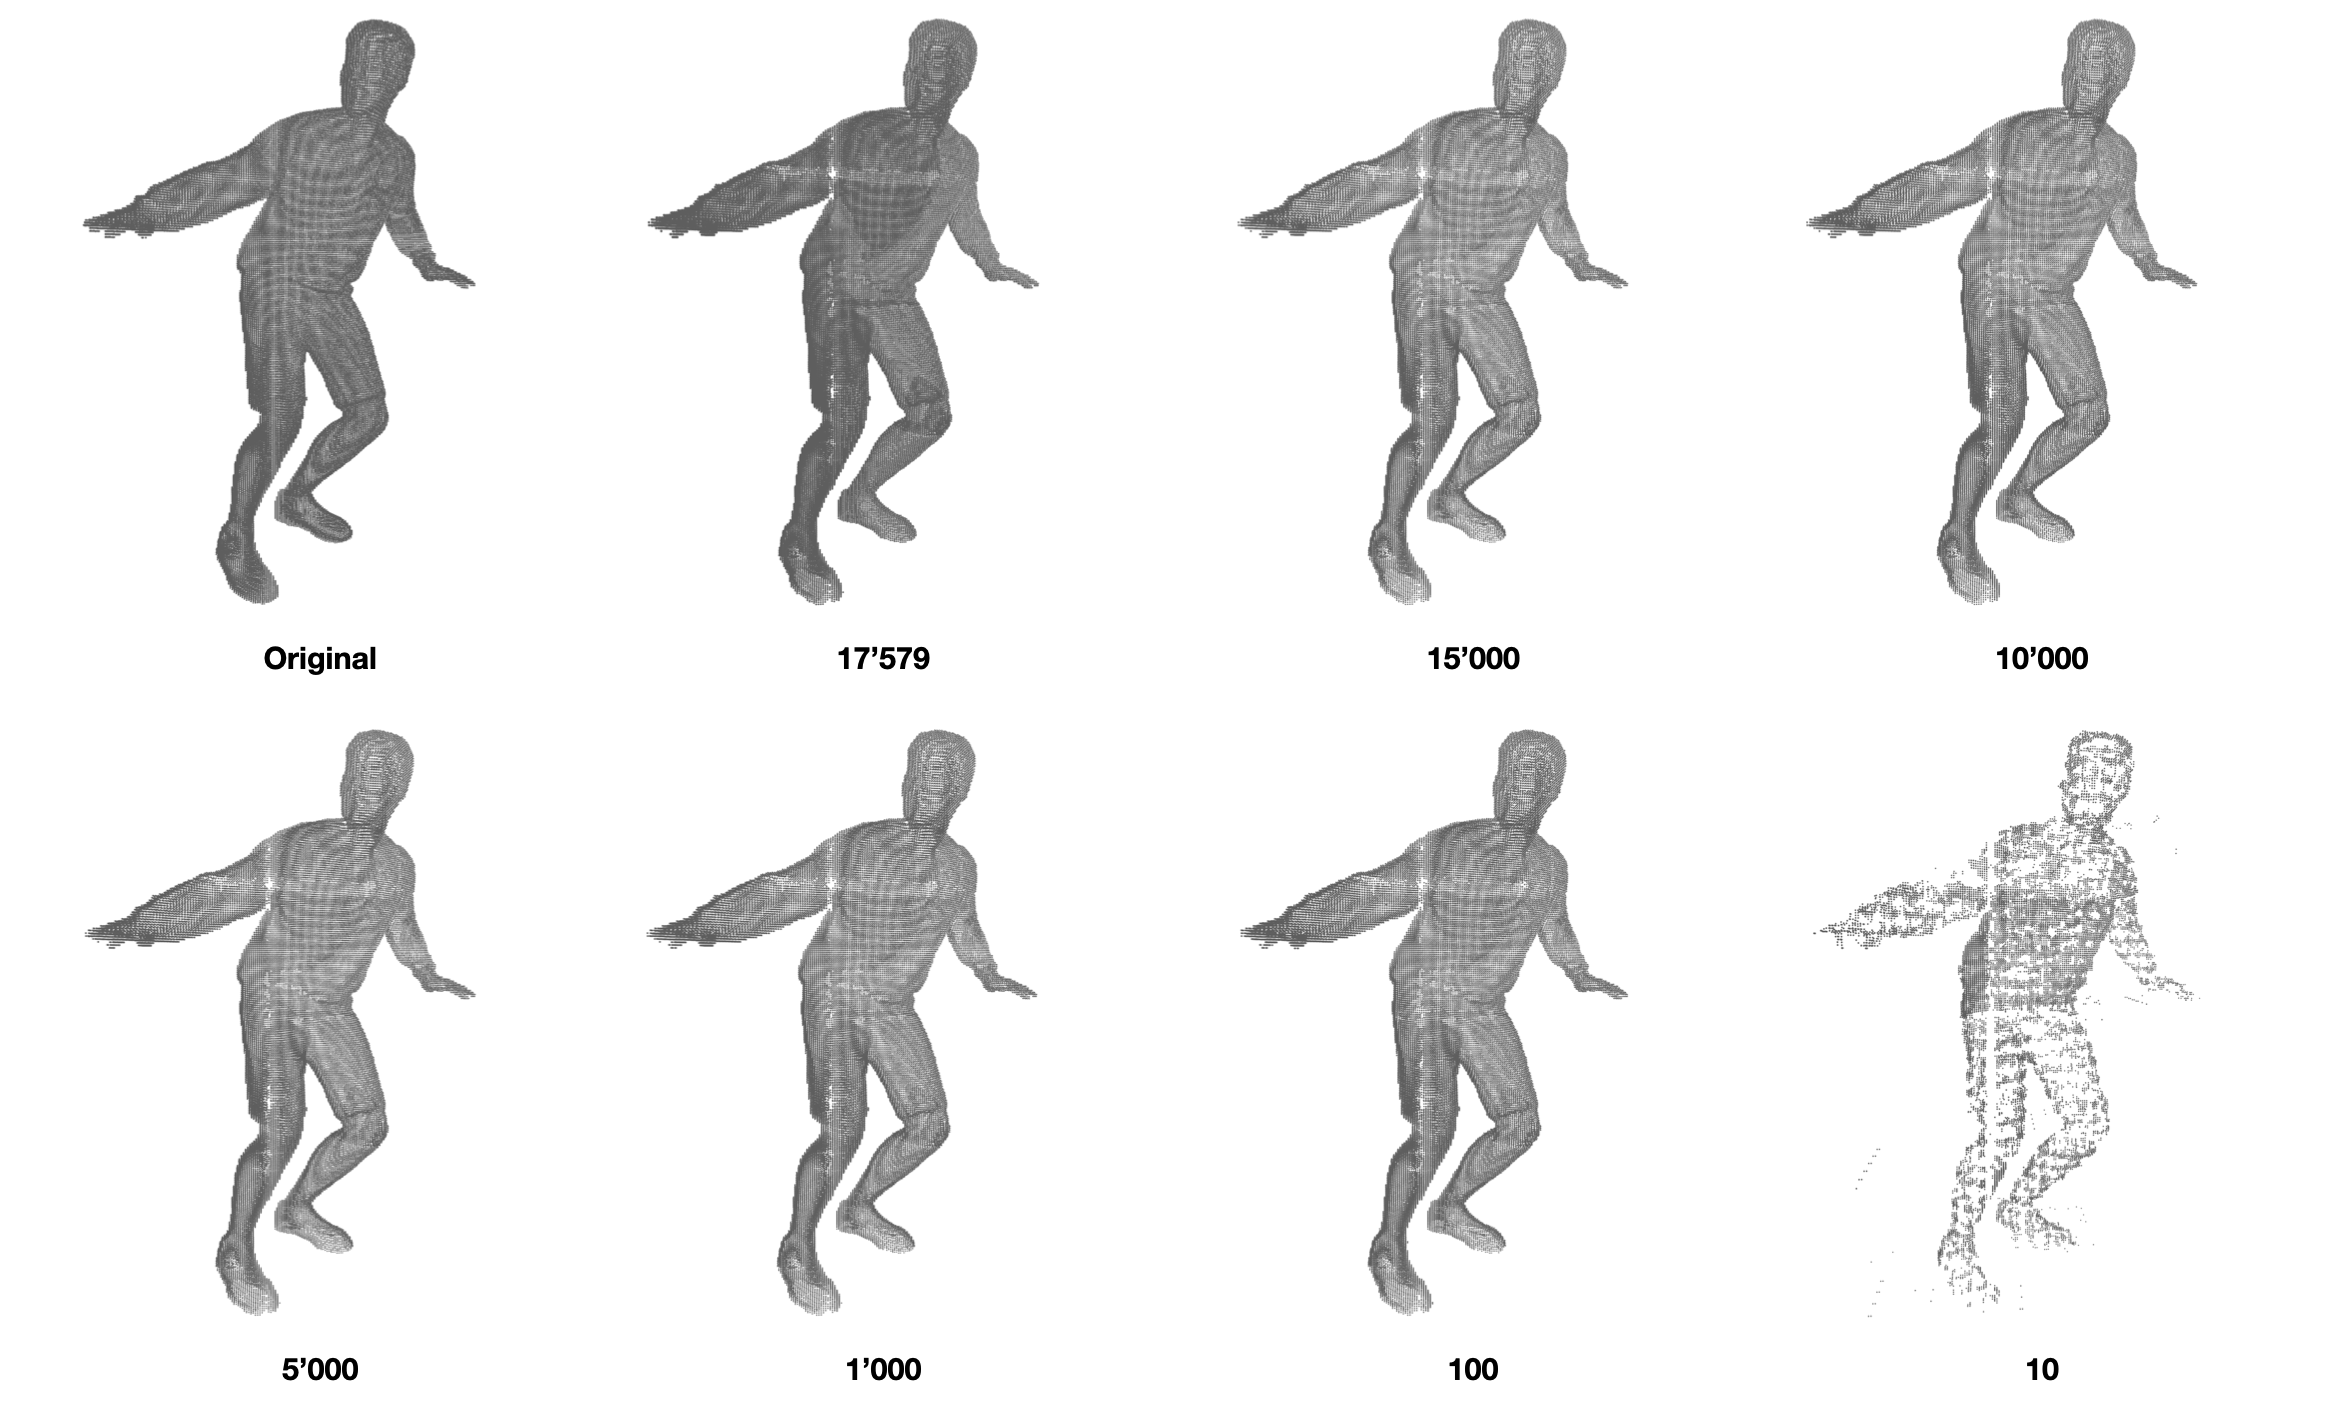
\includegraphics[width=0.9\textwidth]{mesh/all/mitch/results_}
    \caption{Mitch point cloud distortion regarding the span value with a voxelized depth of $8$}
    \label{fig:mitch-all}
\end{figure}

We see some artifacts on the edges of the point cloud blocks, but the distortion is still low. These artifacts are probably due to the linear quantization since it is the only lossy part of the algorithm. The distribution of the latent representation plays a role in these artifacts but we will have a closer look with the rate-distortion analysis.

\section{Rate-distortion analysis}

To evaluate how well the model is performing, we can use a rate-distortion plot to compare how well the model can reconstruct the point cloud at a particular nucleotide rate. With this kind of plot, we can find a trade-off to maximize the reconstruction fidelity while minimizing the number of nucleotides required to encode it.
In this case, the distortion is measured with a D1 PSNR metric which is the PSNR of the point to point MSE between the reconstructed point cloud and the original point cloud (regarding the closest neighbour to each point).

\begin{figure}[ht]
    \centering
    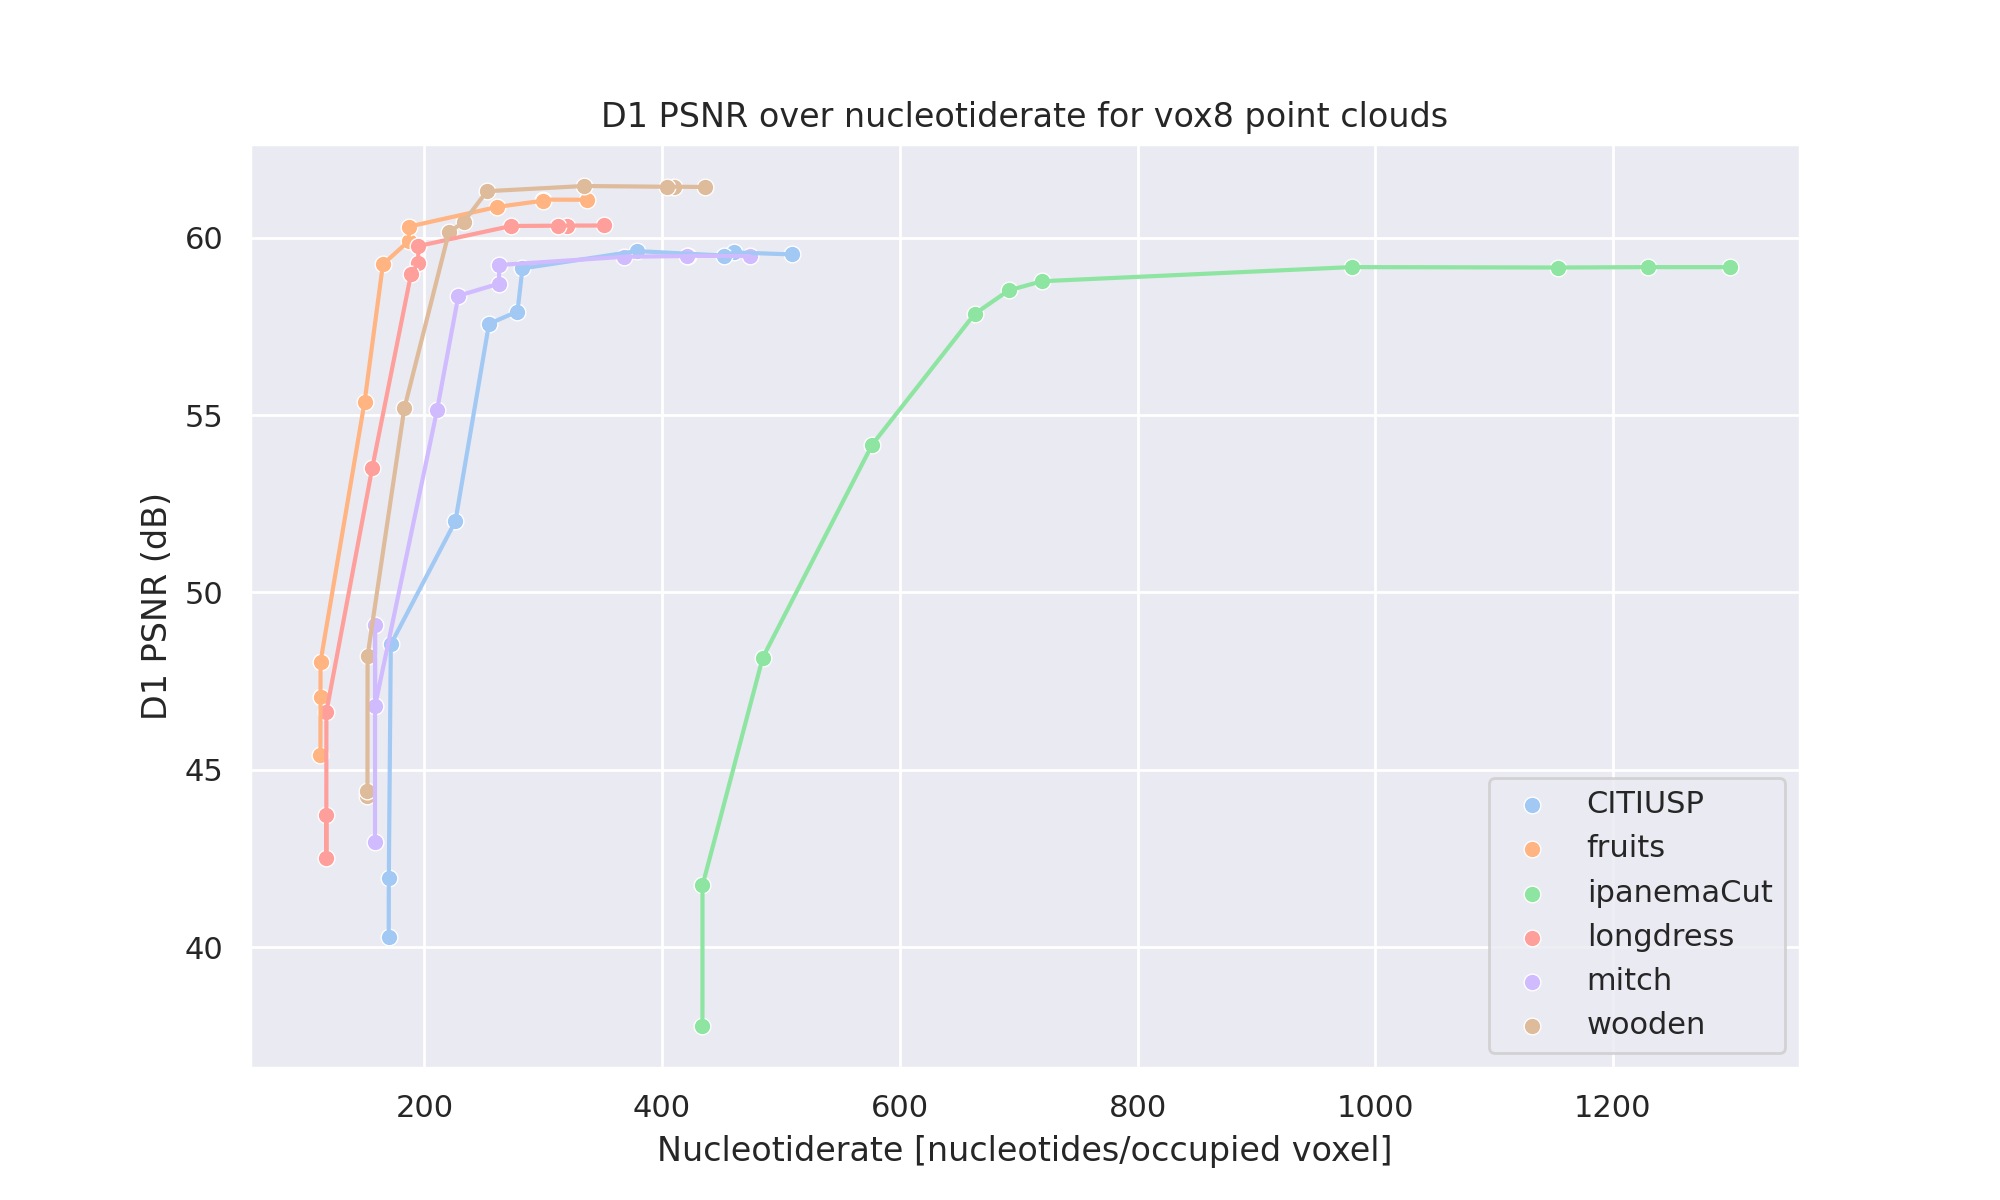
\includegraphics[width=0.9\textwidth]{rate_distortion_span_full2}
    \caption{Rate-distortion analysis regarding the nucleotiderate (controlled by the span value)}
    \label{fig:rate-distortion}
\end{figure}

As we can see in the Figure~\ref{fig:rate-distortion}, the rate-distortion can be easily controlled by the span value. 

These specific nucleotide rates have been computed for the following span values: $$\text{span values} \in \{5, 7, 10, 20, 40, 50, 100, 1000, 5000, 10000, 17579\}$$
We see that the two first span values end up with the same nucleotide rate, while the distortion is much lower for the span value of $7$. We also see that the PSNR is rising quite quickly for the first values without impacting the nucleotide rate much. Both can be explained by the codewords lengths that are small for the first codebooks ($2$ and $3$ codewords lengths) and especially for the span value of $7$, it has $2$ coefficients ($6$ and $7$) that are encoded on length $3$ codewords while the rest is encoded on length $2$ codewords (because falling in the first category codebook). So if the frequency of the $2$ coefficients is not too high, it does not change the final stream length. As we see in the Figure~\ref{fig:quantized-y-1000}, the distribution of the latent representation is not concentrated close to the minimum or the maximum value so there will not be too many extreme values encoded in the final stream.

Weirdly, the ipanemaCut~\ref{fig:ipanema-cut} shows a much higher nucleotide rate than all the others point clouds, it could be explained by the number of occupied voxels that are quite low compared to the overall number of voxels. But the CITIUSP~\ref{fig:citiusp} has a similar structure and has a better nucleotide rate over distortion ratio.

Finally, we can observe that we obtain a maximum PSNR around $60$ quite quickly and that it is no longer increasing with a higher nucleotide rate. It can be explained by the linear quantization that is the only lossy part of the algorithm. Since the distribution of the latent representation is non uniform, as seen on Figure~\ref{fig:quantized-y-1000}, it can explain why the quantization is sub-optimal to turn continuous values into discrete ones.

\begin{figure}[ht]
    \centering
    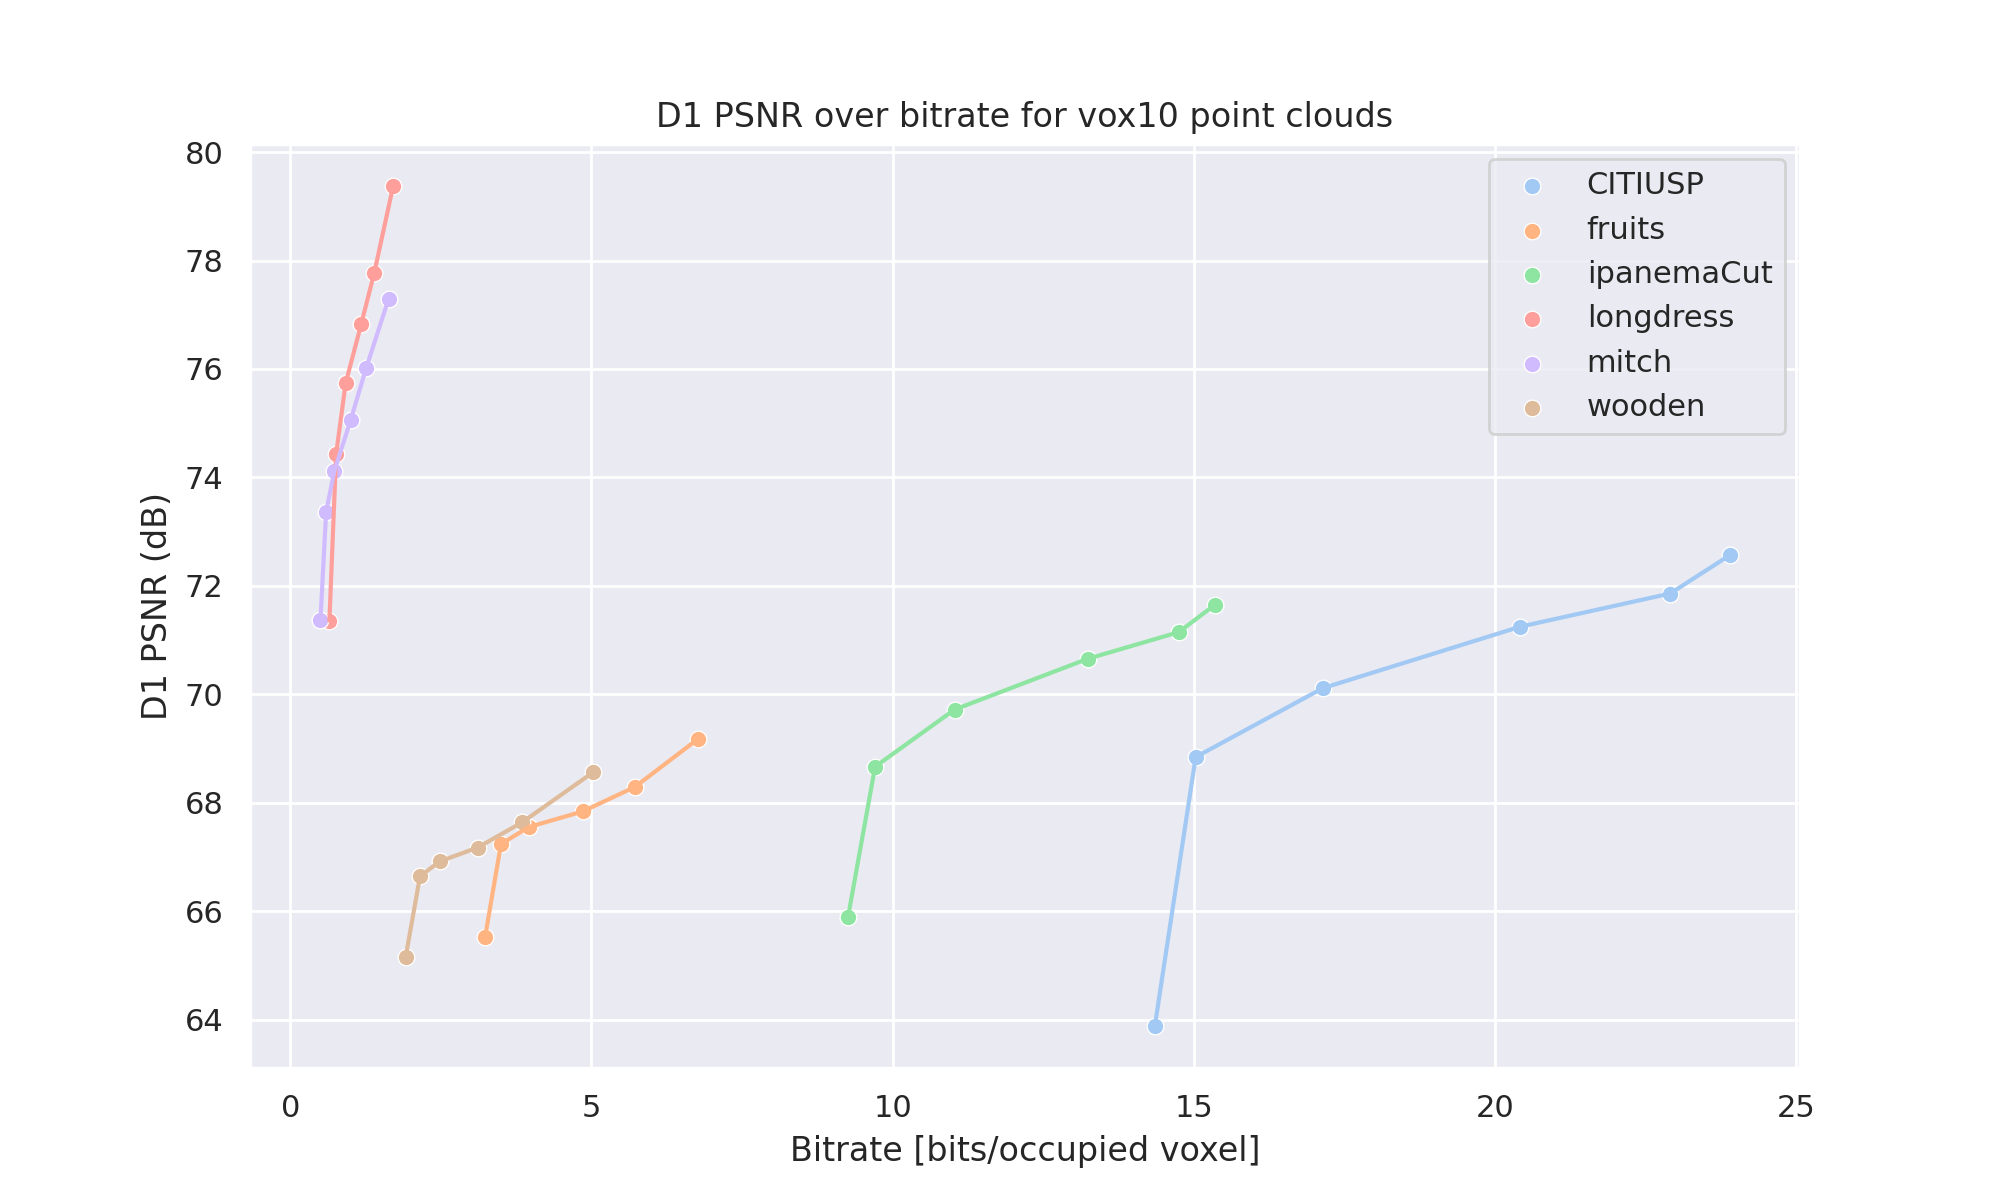
\includegraphics[width=0.9\textwidth]{rate_distortion_standards}
    \caption{Rate-distortion analysis regarding the bitarte for the standard model described in section~\ref{sec:pcc}}
    \label{fig:rate-distortion-standards}
\end{figure}

If we compare with the rate-distortion analysis for the standard model, we can see that the PSNR is higher even with the smallest $\lambda$ value. These bitrates have been computed for the following $\lambda$ values:
$$
\lambda \in \{40,200,400,700,1000,1750\}
$$

We can observe that the bitrate and the distortion depend more on the point cloud that is being encoded than on the DNA version. It is due to the fact that in this case, the latent representation $y$ is entropy encoded per slice, using hyper-analysis entropy parameters and previous slices parameters, which helps a lot quantizing the actual learned distributions per slice. It is thus easily adapted to each point cloud which is not the case of the DNA model since only the whole quantized latent representation is encoded by the JPEG DNA codec. 
Furthermore, the LRP of the standard point cloud compressor helps predicting the error introduced by the quantization and this part is clearly not present in our DNA version, meaning that the quantization is always lost.

If we had wanted to do a naive mapping of the compressed bits to nucleotides, we would have had mapped a single nucleotide every $2$ bits. So we would have ended up with a nucleotide rate of half the bitrate we have on this plot for the same distortion. 
Unfortunately, this naive mapping does not take into account the constraints of the GC-content and homopolymers that are taken into account in the PAIRCODE and Goldman algorithms used in the JPEG DNA codec.

\section{DNA storage simulation}
\label{sec:simu}

In order to see how robust the model is against DNA synthesis, storage and sequencing errors, we will simulate a compressed DNA stream with the MESA simulator. To do that we need to split our full stream into fixed length sequences, called \textit{oligos}. In this simulation we will used the default parameters \ref{yaml:mesa-config} with oligos of length $200$, a storage period of $2$ months, an ErrASE synthesis, $40$ PCR cycles to amplify the oligos, a Taq polymerase and we will store the oligos in a E coli host. With these settings, we can now pass a full \textit{fasta} file to the MESA server that will simulate the full process of synthesis, storage and sequencing and give us back the modified sequences. After merging back together all modified sequences into a single stream, we can pass stream to our decoder that will reconstruct the point cloud from it. 

On the Figure~\ref{fig:simulated-sphere}, you can observe a toy example that has been simulated with the MESA simulator and the parameters specified above. This point cloud is a sphere of size $64 \times 64 \times 64$.

\begin{figure}[ht]
    \centering
    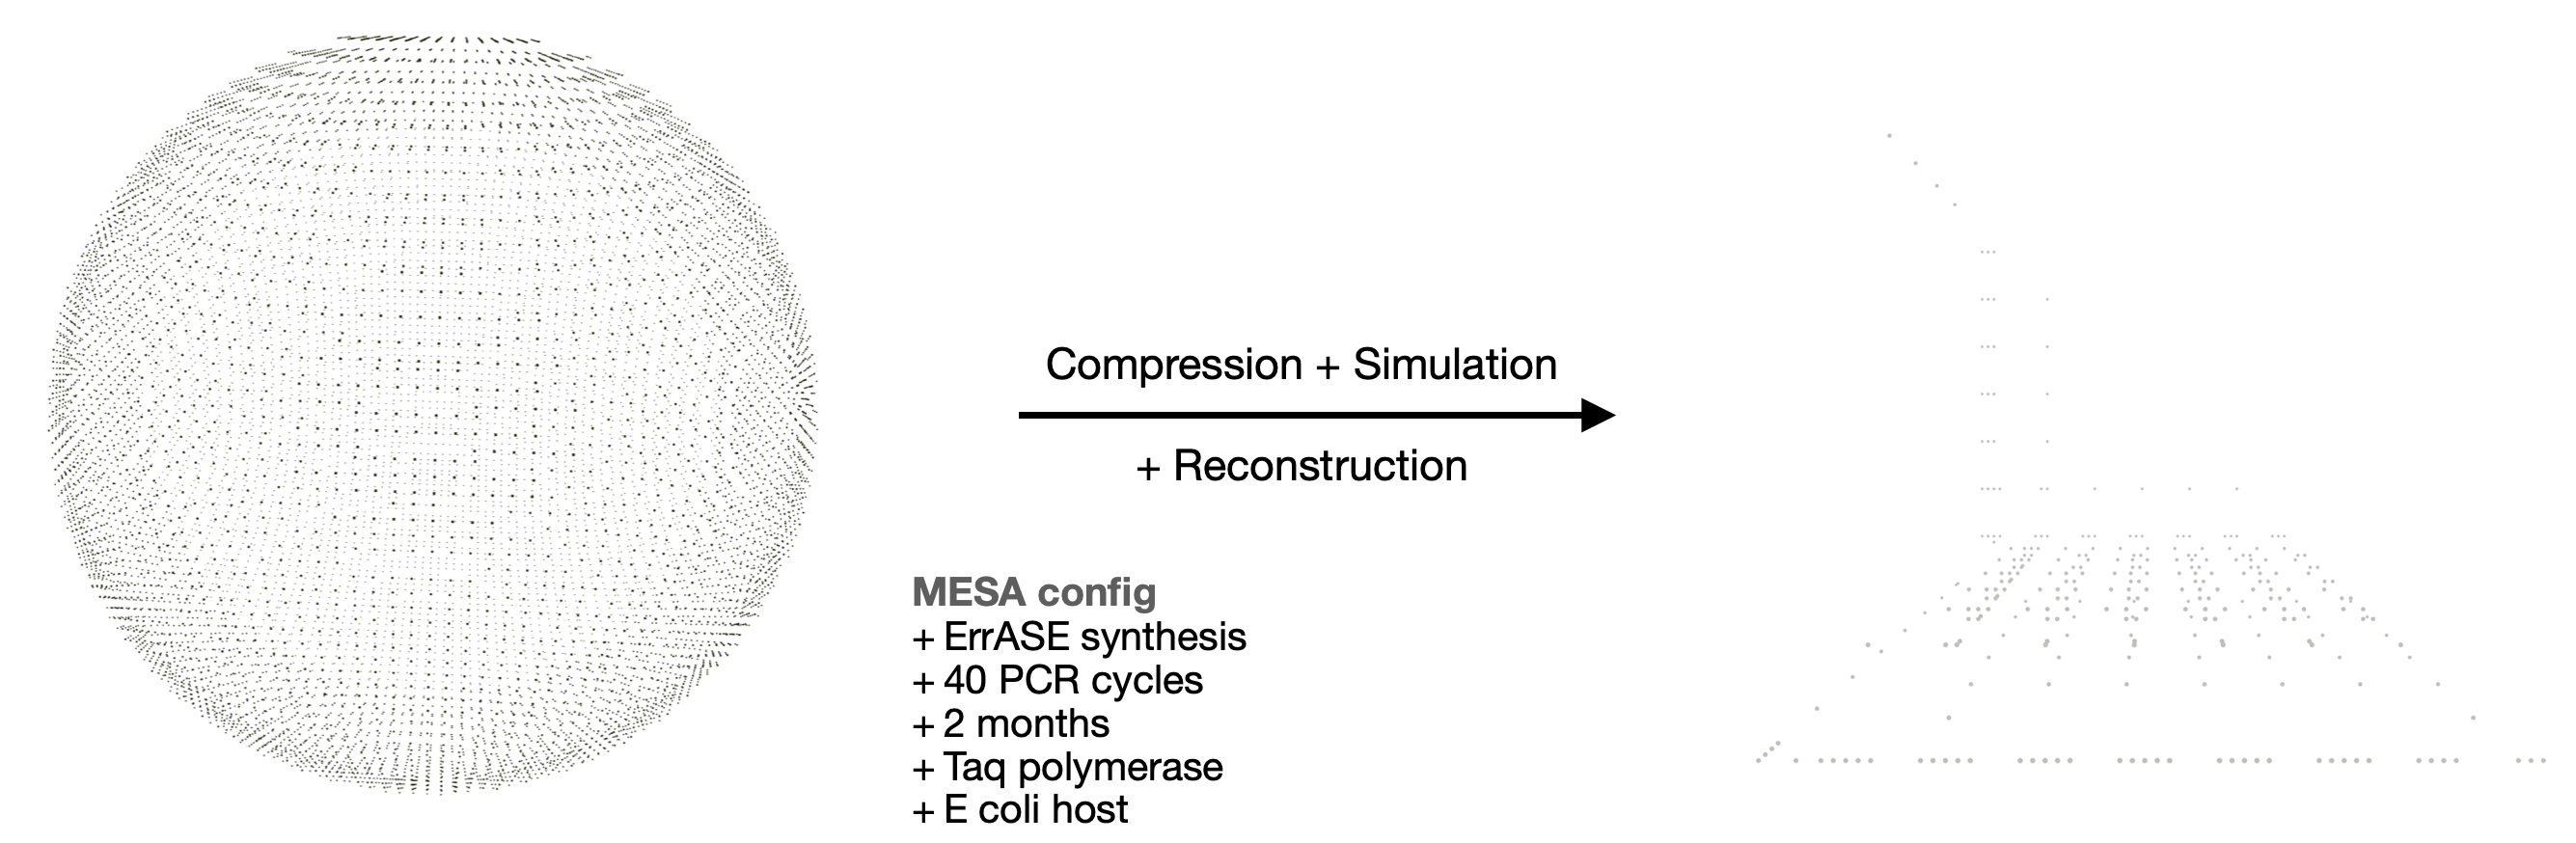
\includegraphics[width=0.9\textwidth]{mesh/sphere_simulation/fig}
    \caption{Simulated DNA stream for a $64$ voxels width sphere}
    \label{fig:simulated-sphere}
\end{figure}

As you can observe, the reconstructed point cloud is not the same as the original one. This is due to the JPEG DNA codec behavior that cannot reconstruct a block if the codeword can not be found in the codebook belonging to the decoded category, in which case it outputs a $8 \times 8$ block of zeros.

\begin{figure}[ht]
    \centering
    \resizebox{0.9\textwidth}{!}{%% Creator: Matplotlib, PGF backend
%%
%% To include the figure in your LaTeX document, write
%%   \input{<filename>.pgf}
%%
%% Make sure the required packages are loaded in your preamble
%%   \usepackage{pgf}
%%
%% Also ensure that all the required font packages are loaded; for instance,
%% the lmodern package is sometimes necessary when using math font.
%%   \usepackage{lmodern}
%%
%% Figures using additional raster images can only be included by \input if
%% they are in the same directory as the main LaTeX file. For loading figures
%% from other directories you can use the `import` package
%%   \usepackage{import}
%%
%% and then include the figures with
%%   \import{<path to file>}{<filename>.pgf}
%%
%% Matplotlib used the following preamble
%%
\begingroup%
\makeatletter%
\begin{pgfpicture}%
\pgfpathrectangle{\pgfpointorigin}{\pgfqpoint{10.000000in}{6.000000in}}%
\pgfusepath{use as bounding box, clip}%
\begin{pgfscope}%
\pgfsetbuttcap%
\pgfsetmiterjoin%
\definecolor{currentfill}{rgb}{1.000000,1.000000,1.000000}%
\pgfsetfillcolor{currentfill}%
\pgfsetlinewidth{0.000000pt}%
\definecolor{currentstroke}{rgb}{1.000000,1.000000,1.000000}%
\pgfsetstrokecolor{currentstroke}%
\pgfsetdash{}{0pt}%
\pgfpathmoveto{\pgfqpoint{0.000000in}{0.000000in}}%
\pgfpathlineto{\pgfqpoint{10.000000in}{0.000000in}}%
\pgfpathlineto{\pgfqpoint{10.000000in}{6.000000in}}%
\pgfpathlineto{\pgfqpoint{0.000000in}{6.000000in}}%
\pgfpathlineto{\pgfqpoint{0.000000in}{0.000000in}}%
\pgfpathclose%
\pgfusepath{fill}%
\end{pgfscope}%
\begin{pgfscope}%
\pgfsetbuttcap%
\pgfsetmiterjoin%
\definecolor{currentfill}{rgb}{0.917647,0.917647,0.949020}%
\pgfsetfillcolor{currentfill}%
\pgfsetlinewidth{0.000000pt}%
\definecolor{currentstroke}{rgb}{0.000000,0.000000,0.000000}%
\pgfsetstrokecolor{currentstroke}%
\pgfsetstrokeopacity{0.000000}%
\pgfsetdash{}{0pt}%
\pgfpathmoveto{\pgfqpoint{1.250000in}{0.660000in}}%
\pgfpathlineto{\pgfqpoint{9.000000in}{0.660000in}}%
\pgfpathlineto{\pgfqpoint{9.000000in}{5.280000in}}%
\pgfpathlineto{\pgfqpoint{1.250000in}{5.280000in}}%
\pgfpathlineto{\pgfqpoint{1.250000in}{0.660000in}}%
\pgfpathclose%
\pgfusepath{fill}%
\end{pgfscope}%
\begin{pgfscope}%
\pgfpathrectangle{\pgfqpoint{1.250000in}{0.660000in}}{\pgfqpoint{7.750000in}{4.620000in}}%
\pgfusepath{clip}%
\pgfsetroundcap%
\pgfsetroundjoin%
\pgfsetlinewidth{1.003750pt}%
\definecolor{currentstroke}{rgb}{1.000000,1.000000,1.000000}%
\pgfsetstrokecolor{currentstroke}%
\pgfsetdash{}{0pt}%
\pgfpathmoveto{\pgfqpoint{1.250000in}{0.660000in}}%
\pgfpathlineto{\pgfqpoint{1.250000in}{5.280000in}}%
\pgfusepath{stroke}%
\end{pgfscope}%
\begin{pgfscope}%
\definecolor{textcolor}{rgb}{0.150000,0.150000,0.150000}%
\pgfsetstrokecolor{textcolor}%
\pgfsetfillcolor{textcolor}%
\pgftext[x=1.250000in,y=0.528056in,,top]{\color{textcolor}\sffamily\fontsize{11.000000}{13.200000}\selectfont \ensuremath{-}35}%
\end{pgfscope}%
\begin{pgfscope}%
\pgfpathrectangle{\pgfqpoint{1.250000in}{0.660000in}}{\pgfqpoint{7.750000in}{4.620000in}}%
\pgfusepath{clip}%
\pgfsetroundcap%
\pgfsetroundjoin%
\pgfsetlinewidth{1.003750pt}%
\definecolor{currentstroke}{rgb}{1.000000,1.000000,1.000000}%
\pgfsetstrokecolor{currentstroke}%
\pgfsetdash{}{0pt}%
\pgfpathmoveto{\pgfqpoint{2.111111in}{0.660000in}}%
\pgfpathlineto{\pgfqpoint{2.111111in}{5.280000in}}%
\pgfusepath{stroke}%
\end{pgfscope}%
\begin{pgfscope}%
\definecolor{textcolor}{rgb}{0.150000,0.150000,0.150000}%
\pgfsetstrokecolor{textcolor}%
\pgfsetfillcolor{textcolor}%
\pgftext[x=2.111111in,y=0.528056in,,top]{\color{textcolor}\sffamily\fontsize{11.000000}{13.200000}\selectfont \ensuremath{-}30}%
\end{pgfscope}%
\begin{pgfscope}%
\pgfpathrectangle{\pgfqpoint{1.250000in}{0.660000in}}{\pgfqpoint{7.750000in}{4.620000in}}%
\pgfusepath{clip}%
\pgfsetroundcap%
\pgfsetroundjoin%
\pgfsetlinewidth{1.003750pt}%
\definecolor{currentstroke}{rgb}{1.000000,1.000000,1.000000}%
\pgfsetstrokecolor{currentstroke}%
\pgfsetdash{}{0pt}%
\pgfpathmoveto{\pgfqpoint{2.972222in}{0.660000in}}%
\pgfpathlineto{\pgfqpoint{2.972222in}{5.280000in}}%
\pgfusepath{stroke}%
\end{pgfscope}%
\begin{pgfscope}%
\definecolor{textcolor}{rgb}{0.150000,0.150000,0.150000}%
\pgfsetstrokecolor{textcolor}%
\pgfsetfillcolor{textcolor}%
\pgftext[x=2.972222in,y=0.528056in,,top]{\color{textcolor}\sffamily\fontsize{11.000000}{13.200000}\selectfont \ensuremath{-}25}%
\end{pgfscope}%
\begin{pgfscope}%
\pgfpathrectangle{\pgfqpoint{1.250000in}{0.660000in}}{\pgfqpoint{7.750000in}{4.620000in}}%
\pgfusepath{clip}%
\pgfsetroundcap%
\pgfsetroundjoin%
\pgfsetlinewidth{1.003750pt}%
\definecolor{currentstroke}{rgb}{1.000000,1.000000,1.000000}%
\pgfsetstrokecolor{currentstroke}%
\pgfsetdash{}{0pt}%
\pgfpathmoveto{\pgfqpoint{3.833333in}{0.660000in}}%
\pgfpathlineto{\pgfqpoint{3.833333in}{5.280000in}}%
\pgfusepath{stroke}%
\end{pgfscope}%
\begin{pgfscope}%
\definecolor{textcolor}{rgb}{0.150000,0.150000,0.150000}%
\pgfsetstrokecolor{textcolor}%
\pgfsetfillcolor{textcolor}%
\pgftext[x=3.833333in,y=0.528056in,,top]{\color{textcolor}\sffamily\fontsize{11.000000}{13.200000}\selectfont \ensuremath{-}20}%
\end{pgfscope}%
\begin{pgfscope}%
\pgfpathrectangle{\pgfqpoint{1.250000in}{0.660000in}}{\pgfqpoint{7.750000in}{4.620000in}}%
\pgfusepath{clip}%
\pgfsetroundcap%
\pgfsetroundjoin%
\pgfsetlinewidth{1.003750pt}%
\definecolor{currentstroke}{rgb}{1.000000,1.000000,1.000000}%
\pgfsetstrokecolor{currentstroke}%
\pgfsetdash{}{0pt}%
\pgfpathmoveto{\pgfqpoint{4.694444in}{0.660000in}}%
\pgfpathlineto{\pgfqpoint{4.694444in}{5.280000in}}%
\pgfusepath{stroke}%
\end{pgfscope}%
\begin{pgfscope}%
\definecolor{textcolor}{rgb}{0.150000,0.150000,0.150000}%
\pgfsetstrokecolor{textcolor}%
\pgfsetfillcolor{textcolor}%
\pgftext[x=4.694444in,y=0.528056in,,top]{\color{textcolor}\sffamily\fontsize{11.000000}{13.200000}\selectfont \ensuremath{-}15}%
\end{pgfscope}%
\begin{pgfscope}%
\pgfpathrectangle{\pgfqpoint{1.250000in}{0.660000in}}{\pgfqpoint{7.750000in}{4.620000in}}%
\pgfusepath{clip}%
\pgfsetroundcap%
\pgfsetroundjoin%
\pgfsetlinewidth{1.003750pt}%
\definecolor{currentstroke}{rgb}{1.000000,1.000000,1.000000}%
\pgfsetstrokecolor{currentstroke}%
\pgfsetdash{}{0pt}%
\pgfpathmoveto{\pgfqpoint{5.555556in}{0.660000in}}%
\pgfpathlineto{\pgfqpoint{5.555556in}{5.280000in}}%
\pgfusepath{stroke}%
\end{pgfscope}%
\begin{pgfscope}%
\definecolor{textcolor}{rgb}{0.150000,0.150000,0.150000}%
\pgfsetstrokecolor{textcolor}%
\pgfsetfillcolor{textcolor}%
\pgftext[x=5.555556in,y=0.528056in,,top]{\color{textcolor}\sffamily\fontsize{11.000000}{13.200000}\selectfont \ensuremath{-}10}%
\end{pgfscope}%
\begin{pgfscope}%
\pgfpathrectangle{\pgfqpoint{1.250000in}{0.660000in}}{\pgfqpoint{7.750000in}{4.620000in}}%
\pgfusepath{clip}%
\pgfsetroundcap%
\pgfsetroundjoin%
\pgfsetlinewidth{1.003750pt}%
\definecolor{currentstroke}{rgb}{1.000000,1.000000,1.000000}%
\pgfsetstrokecolor{currentstroke}%
\pgfsetdash{}{0pt}%
\pgfpathmoveto{\pgfqpoint{6.416667in}{0.660000in}}%
\pgfpathlineto{\pgfqpoint{6.416667in}{5.280000in}}%
\pgfusepath{stroke}%
\end{pgfscope}%
\begin{pgfscope}%
\definecolor{textcolor}{rgb}{0.150000,0.150000,0.150000}%
\pgfsetstrokecolor{textcolor}%
\pgfsetfillcolor{textcolor}%
\pgftext[x=6.416667in,y=0.528056in,,top]{\color{textcolor}\sffamily\fontsize{11.000000}{13.200000}\selectfont \ensuremath{-}5}%
\end{pgfscope}%
\begin{pgfscope}%
\pgfpathrectangle{\pgfqpoint{1.250000in}{0.660000in}}{\pgfqpoint{7.750000in}{4.620000in}}%
\pgfusepath{clip}%
\pgfsetroundcap%
\pgfsetroundjoin%
\pgfsetlinewidth{1.003750pt}%
\definecolor{currentstroke}{rgb}{1.000000,1.000000,1.000000}%
\pgfsetstrokecolor{currentstroke}%
\pgfsetdash{}{0pt}%
\pgfpathmoveto{\pgfqpoint{7.277778in}{0.660000in}}%
\pgfpathlineto{\pgfqpoint{7.277778in}{5.280000in}}%
\pgfusepath{stroke}%
\end{pgfscope}%
\begin{pgfscope}%
\definecolor{textcolor}{rgb}{0.150000,0.150000,0.150000}%
\pgfsetstrokecolor{textcolor}%
\pgfsetfillcolor{textcolor}%
\pgftext[x=7.277778in,y=0.528056in,,top]{\color{textcolor}\sffamily\fontsize{11.000000}{13.200000}\selectfont 0}%
\end{pgfscope}%
\begin{pgfscope}%
\pgfpathrectangle{\pgfqpoint{1.250000in}{0.660000in}}{\pgfqpoint{7.750000in}{4.620000in}}%
\pgfusepath{clip}%
\pgfsetroundcap%
\pgfsetroundjoin%
\pgfsetlinewidth{1.003750pt}%
\definecolor{currentstroke}{rgb}{1.000000,1.000000,1.000000}%
\pgfsetstrokecolor{currentstroke}%
\pgfsetdash{}{0pt}%
\pgfpathmoveto{\pgfqpoint{8.138889in}{0.660000in}}%
\pgfpathlineto{\pgfqpoint{8.138889in}{5.280000in}}%
\pgfusepath{stroke}%
\end{pgfscope}%
\begin{pgfscope}%
\definecolor{textcolor}{rgb}{0.150000,0.150000,0.150000}%
\pgfsetstrokecolor{textcolor}%
\pgfsetfillcolor{textcolor}%
\pgftext[x=8.138889in,y=0.528056in,,top]{\color{textcolor}\sffamily\fontsize{11.000000}{13.200000}\selectfont 5}%
\end{pgfscope}%
\begin{pgfscope}%
\pgfpathrectangle{\pgfqpoint{1.250000in}{0.660000in}}{\pgfqpoint{7.750000in}{4.620000in}}%
\pgfusepath{clip}%
\pgfsetroundcap%
\pgfsetroundjoin%
\pgfsetlinewidth{1.003750pt}%
\definecolor{currentstroke}{rgb}{1.000000,1.000000,1.000000}%
\pgfsetstrokecolor{currentstroke}%
\pgfsetdash{}{0pt}%
\pgfpathmoveto{\pgfqpoint{9.000000in}{0.660000in}}%
\pgfpathlineto{\pgfqpoint{9.000000in}{5.280000in}}%
\pgfusepath{stroke}%
\end{pgfscope}%
\begin{pgfscope}%
\definecolor{textcolor}{rgb}{0.150000,0.150000,0.150000}%
\pgfsetstrokecolor{textcolor}%
\pgfsetfillcolor{textcolor}%
\pgftext[x=9.000000in,y=0.528056in,,top]{\color{textcolor}\sffamily\fontsize{11.000000}{13.200000}\selectfont 10}%
\end{pgfscope}%
\begin{pgfscope}%
\definecolor{textcolor}{rgb}{0.150000,0.150000,0.150000}%
\pgfsetstrokecolor{textcolor}%
\pgfsetfillcolor{textcolor}%
\pgftext[x=5.125000in,y=0.337315in,,top]{\color{textcolor}\sffamily\fontsize{12.000000}{14.400000}\selectfont Latent representation values}%
\end{pgfscope}%
\begin{pgfscope}%
\pgfpathrectangle{\pgfqpoint{1.250000in}{0.660000in}}{\pgfqpoint{7.750000in}{4.620000in}}%
\pgfusepath{clip}%
\pgfsetroundcap%
\pgfsetroundjoin%
\pgfsetlinewidth{1.003750pt}%
\definecolor{currentstroke}{rgb}{1.000000,1.000000,1.000000}%
\pgfsetstrokecolor{currentstroke}%
\pgfsetdash{}{0pt}%
\pgfpathmoveto{\pgfqpoint{1.250000in}{0.660000in}}%
\pgfpathlineto{\pgfqpoint{9.000000in}{0.660000in}}%
\pgfusepath{stroke}%
\end{pgfscope}%
\begin{pgfscope}%
\definecolor{textcolor}{rgb}{0.150000,0.150000,0.150000}%
\pgfsetstrokecolor{textcolor}%
\pgfsetfillcolor{textcolor}%
\pgftext[x=0.923727in, y=0.607193in, left, base]{\color{textcolor}\sffamily\fontsize{11.000000}{13.200000}\selectfont 0.0}%
\end{pgfscope}%
\begin{pgfscope}%
\pgfpathrectangle{\pgfqpoint{1.250000in}{0.660000in}}{\pgfqpoint{7.750000in}{4.620000in}}%
\pgfusepath{clip}%
\pgfsetroundcap%
\pgfsetroundjoin%
\pgfsetlinewidth{1.003750pt}%
\definecolor{currentstroke}{rgb}{1.000000,1.000000,1.000000}%
\pgfsetstrokecolor{currentstroke}%
\pgfsetdash{}{0pt}%
\pgfpathmoveto{\pgfqpoint{1.250000in}{1.662067in}}%
\pgfpathlineto{\pgfqpoint{9.000000in}{1.662067in}}%
\pgfusepath{stroke}%
\end{pgfscope}%
\begin{pgfscope}%
\definecolor{textcolor}{rgb}{0.150000,0.150000,0.150000}%
\pgfsetstrokecolor{textcolor}%
\pgfsetfillcolor{textcolor}%
\pgftext[x=0.923727in, y=1.609261in, left, base]{\color{textcolor}\sffamily\fontsize{11.000000}{13.200000}\selectfont 0.2}%
\end{pgfscope}%
\begin{pgfscope}%
\pgfpathrectangle{\pgfqpoint{1.250000in}{0.660000in}}{\pgfqpoint{7.750000in}{4.620000in}}%
\pgfusepath{clip}%
\pgfsetroundcap%
\pgfsetroundjoin%
\pgfsetlinewidth{1.003750pt}%
\definecolor{currentstroke}{rgb}{1.000000,1.000000,1.000000}%
\pgfsetstrokecolor{currentstroke}%
\pgfsetdash{}{0pt}%
\pgfpathmoveto{\pgfqpoint{1.250000in}{2.664135in}}%
\pgfpathlineto{\pgfqpoint{9.000000in}{2.664135in}}%
\pgfusepath{stroke}%
\end{pgfscope}%
\begin{pgfscope}%
\definecolor{textcolor}{rgb}{0.150000,0.150000,0.150000}%
\pgfsetstrokecolor{textcolor}%
\pgfsetfillcolor{textcolor}%
\pgftext[x=0.923727in, y=2.611328in, left, base]{\color{textcolor}\sffamily\fontsize{11.000000}{13.200000}\selectfont 0.4}%
\end{pgfscope}%
\begin{pgfscope}%
\pgfpathrectangle{\pgfqpoint{1.250000in}{0.660000in}}{\pgfqpoint{7.750000in}{4.620000in}}%
\pgfusepath{clip}%
\pgfsetroundcap%
\pgfsetroundjoin%
\pgfsetlinewidth{1.003750pt}%
\definecolor{currentstroke}{rgb}{1.000000,1.000000,1.000000}%
\pgfsetstrokecolor{currentstroke}%
\pgfsetdash{}{0pt}%
\pgfpathmoveto{\pgfqpoint{1.250000in}{3.666202in}}%
\pgfpathlineto{\pgfqpoint{9.000000in}{3.666202in}}%
\pgfusepath{stroke}%
\end{pgfscope}%
\begin{pgfscope}%
\definecolor{textcolor}{rgb}{0.150000,0.150000,0.150000}%
\pgfsetstrokecolor{textcolor}%
\pgfsetfillcolor{textcolor}%
\pgftext[x=0.923727in, y=3.613396in, left, base]{\color{textcolor}\sffamily\fontsize{11.000000}{13.200000}\selectfont 0.6}%
\end{pgfscope}%
\begin{pgfscope}%
\pgfpathrectangle{\pgfqpoint{1.250000in}{0.660000in}}{\pgfqpoint{7.750000in}{4.620000in}}%
\pgfusepath{clip}%
\pgfsetroundcap%
\pgfsetroundjoin%
\pgfsetlinewidth{1.003750pt}%
\definecolor{currentstroke}{rgb}{1.000000,1.000000,1.000000}%
\pgfsetstrokecolor{currentstroke}%
\pgfsetdash{}{0pt}%
\pgfpathmoveto{\pgfqpoint{1.250000in}{4.668270in}}%
\pgfpathlineto{\pgfqpoint{9.000000in}{4.668270in}}%
\pgfusepath{stroke}%
\end{pgfscope}%
\begin{pgfscope}%
\definecolor{textcolor}{rgb}{0.150000,0.150000,0.150000}%
\pgfsetstrokecolor{textcolor}%
\pgfsetfillcolor{textcolor}%
\pgftext[x=0.923727in, y=4.615463in, left, base]{\color{textcolor}\sffamily\fontsize{11.000000}{13.200000}\selectfont 0.8}%
\end{pgfscope}%
\begin{pgfscope}%
\definecolor{textcolor}{rgb}{0.150000,0.150000,0.150000}%
\pgfsetstrokecolor{textcolor}%
\pgfsetfillcolor{textcolor}%
\pgftext[x=0.868171in,y=2.970000in,,bottom,rotate=90.000000]{\color{textcolor}\sffamily\fontsize{12.000000}{14.400000}\selectfont Density}%
\end{pgfscope}%
\begin{pgfscope}%
\pgfpathrectangle{\pgfqpoint{1.250000in}{0.660000in}}{\pgfqpoint{7.750000in}{4.620000in}}%
\pgfusepath{clip}%
\pgfsetbuttcap%
\pgfsetroundjoin%
\definecolor{currentfill}{rgb}{0.312703,0.620721,0.563793}%
\pgfsetfillcolor{currentfill}%
\pgfsetfillopacity{0.250000}%
\pgfsetlinewidth{1.003750pt}%
\definecolor{currentstroke}{rgb}{0.312703,0.620721,0.563793}%
\pgfsetstrokecolor{currentstroke}%
\pgfsetdash{}{0pt}%
\pgfpathmoveto{\pgfqpoint{1.935494in}{0.660001in}}%
\pgfpathlineto{\pgfqpoint{1.935494in}{0.660000in}}%
\pgfpathlineto{\pgfqpoint{2.000424in}{0.660000in}}%
\pgfpathlineto{\pgfqpoint{2.065354in}{0.660000in}}%
\pgfpathlineto{\pgfqpoint{2.130285in}{0.660000in}}%
\pgfpathlineto{\pgfqpoint{2.195215in}{0.660000in}}%
\pgfpathlineto{\pgfqpoint{2.260145in}{0.660000in}}%
\pgfpathlineto{\pgfqpoint{2.325076in}{0.660000in}}%
\pgfpathlineto{\pgfqpoint{2.390006in}{0.660000in}}%
\pgfpathlineto{\pgfqpoint{2.454936in}{0.660000in}}%
\pgfpathlineto{\pgfqpoint{2.519866in}{0.660000in}}%
\pgfpathlineto{\pgfqpoint{2.584797in}{0.660000in}}%
\pgfpathlineto{\pgfqpoint{2.649727in}{0.660000in}}%
\pgfpathlineto{\pgfqpoint{2.714657in}{0.660000in}}%
\pgfpathlineto{\pgfqpoint{2.779588in}{0.660000in}}%
\pgfpathlineto{\pgfqpoint{2.844518in}{0.660000in}}%
\pgfpathlineto{\pgfqpoint{2.909448in}{0.660000in}}%
\pgfpathlineto{\pgfqpoint{2.974379in}{0.660000in}}%
\pgfpathlineto{\pgfqpoint{3.039309in}{0.660000in}}%
\pgfpathlineto{\pgfqpoint{3.104239in}{0.660000in}}%
\pgfpathlineto{\pgfqpoint{3.169170in}{0.660000in}}%
\pgfpathlineto{\pgfqpoint{3.234100in}{0.660000in}}%
\pgfpathlineto{\pgfqpoint{3.299030in}{0.660000in}}%
\pgfpathlineto{\pgfqpoint{3.363961in}{0.660000in}}%
\pgfpathlineto{\pgfqpoint{3.428891in}{0.660000in}}%
\pgfpathlineto{\pgfqpoint{3.493821in}{0.660000in}}%
\pgfpathlineto{\pgfqpoint{3.558751in}{0.660000in}}%
\pgfpathlineto{\pgfqpoint{3.623682in}{0.660000in}}%
\pgfpathlineto{\pgfqpoint{3.688612in}{0.660000in}}%
\pgfpathlineto{\pgfqpoint{3.753542in}{0.660000in}}%
\pgfpathlineto{\pgfqpoint{3.818473in}{0.660000in}}%
\pgfpathlineto{\pgfqpoint{3.883403in}{0.660000in}}%
\pgfpathlineto{\pgfqpoint{3.948333in}{0.660000in}}%
\pgfpathlineto{\pgfqpoint{4.013264in}{0.660000in}}%
\pgfpathlineto{\pgfqpoint{4.078194in}{0.660000in}}%
\pgfpathlineto{\pgfqpoint{4.143124in}{0.660000in}}%
\pgfpathlineto{\pgfqpoint{4.208055in}{0.660000in}}%
\pgfpathlineto{\pgfqpoint{4.272985in}{0.660000in}}%
\pgfpathlineto{\pgfqpoint{4.337915in}{0.660000in}}%
\pgfpathlineto{\pgfqpoint{4.402845in}{0.660000in}}%
\pgfpathlineto{\pgfqpoint{4.467776in}{0.660000in}}%
\pgfpathlineto{\pgfqpoint{4.532706in}{0.660000in}}%
\pgfpathlineto{\pgfqpoint{4.597636in}{0.660000in}}%
\pgfpathlineto{\pgfqpoint{4.662567in}{0.660000in}}%
\pgfpathlineto{\pgfqpoint{4.727497in}{0.660000in}}%
\pgfpathlineto{\pgfqpoint{4.792427in}{0.660000in}}%
\pgfpathlineto{\pgfqpoint{4.857358in}{0.660000in}}%
\pgfpathlineto{\pgfqpoint{4.922288in}{0.660000in}}%
\pgfpathlineto{\pgfqpoint{4.987218in}{0.660000in}}%
\pgfpathlineto{\pgfqpoint{5.052149in}{0.660000in}}%
\pgfpathlineto{\pgfqpoint{5.117079in}{0.660000in}}%
\pgfpathlineto{\pgfqpoint{5.182009in}{0.660000in}}%
\pgfpathlineto{\pgfqpoint{5.246939in}{0.660000in}}%
\pgfpathlineto{\pgfqpoint{5.311870in}{0.660000in}}%
\pgfpathlineto{\pgfqpoint{5.376800in}{0.660000in}}%
\pgfpathlineto{\pgfqpoint{5.441730in}{0.660000in}}%
\pgfpathlineto{\pgfqpoint{5.506661in}{0.660000in}}%
\pgfpathlineto{\pgfqpoint{5.571591in}{0.660000in}}%
\pgfpathlineto{\pgfqpoint{5.636521in}{0.660000in}}%
\pgfpathlineto{\pgfqpoint{5.701452in}{0.660000in}}%
\pgfpathlineto{\pgfqpoint{5.766382in}{0.660000in}}%
\pgfpathlineto{\pgfqpoint{5.831312in}{0.660000in}}%
\pgfpathlineto{\pgfqpoint{5.896243in}{0.660000in}}%
\pgfpathlineto{\pgfqpoint{5.961173in}{0.660000in}}%
\pgfpathlineto{\pgfqpoint{6.026103in}{0.660000in}}%
\pgfpathlineto{\pgfqpoint{6.091034in}{0.660000in}}%
\pgfpathlineto{\pgfqpoint{6.155964in}{0.660000in}}%
\pgfpathlineto{\pgfqpoint{6.220894in}{0.660000in}}%
\pgfpathlineto{\pgfqpoint{6.285824in}{0.660000in}}%
\pgfpathlineto{\pgfqpoint{6.350755in}{0.660000in}}%
\pgfpathlineto{\pgfqpoint{6.415685in}{0.660000in}}%
\pgfpathlineto{\pgfqpoint{6.480615in}{0.660000in}}%
\pgfpathlineto{\pgfqpoint{6.545546in}{0.660000in}}%
\pgfpathlineto{\pgfqpoint{6.610476in}{0.660000in}}%
\pgfpathlineto{\pgfqpoint{6.675406in}{0.660000in}}%
\pgfpathlineto{\pgfqpoint{6.740337in}{0.660000in}}%
\pgfpathlineto{\pgfqpoint{6.805267in}{0.660000in}}%
\pgfpathlineto{\pgfqpoint{6.870197in}{0.660000in}}%
\pgfpathlineto{\pgfqpoint{6.935128in}{0.660000in}}%
\pgfpathlineto{\pgfqpoint{7.000058in}{0.660000in}}%
\pgfpathlineto{\pgfqpoint{7.064988in}{0.660000in}}%
\pgfpathlineto{\pgfqpoint{7.129918in}{0.660000in}}%
\pgfpathlineto{\pgfqpoint{7.194849in}{0.660000in}}%
\pgfpathlineto{\pgfqpoint{7.259779in}{0.660000in}}%
\pgfpathlineto{\pgfqpoint{7.324709in}{0.660000in}}%
\pgfpathlineto{\pgfqpoint{7.389640in}{0.660000in}}%
\pgfpathlineto{\pgfqpoint{7.454570in}{0.660000in}}%
\pgfpathlineto{\pgfqpoint{7.519500in}{0.660000in}}%
\pgfpathlineto{\pgfqpoint{7.584431in}{0.660000in}}%
\pgfpathlineto{\pgfqpoint{7.649361in}{0.660000in}}%
\pgfpathlineto{\pgfqpoint{7.714291in}{0.660000in}}%
\pgfpathlineto{\pgfqpoint{7.779222in}{0.660000in}}%
\pgfpathlineto{\pgfqpoint{7.844152in}{0.660000in}}%
\pgfpathlineto{\pgfqpoint{7.909082in}{0.660000in}}%
\pgfpathlineto{\pgfqpoint{7.974013in}{0.660000in}}%
\pgfpathlineto{\pgfqpoint{8.038943in}{0.660000in}}%
\pgfpathlineto{\pgfqpoint{8.103873in}{0.660000in}}%
\pgfpathlineto{\pgfqpoint{8.168803in}{0.660000in}}%
\pgfpathlineto{\pgfqpoint{8.233734in}{0.660000in}}%
\pgfpathlineto{\pgfqpoint{8.298664in}{0.660000in}}%
\pgfpathlineto{\pgfqpoint{8.363594in}{0.660000in}}%
\pgfpathlineto{\pgfqpoint{8.428525in}{0.660000in}}%
\pgfpathlineto{\pgfqpoint{8.493455in}{0.660000in}}%
\pgfpathlineto{\pgfqpoint{8.558385in}{0.660000in}}%
\pgfpathlineto{\pgfqpoint{8.623316in}{0.660000in}}%
\pgfpathlineto{\pgfqpoint{8.688246in}{0.660000in}}%
\pgfpathlineto{\pgfqpoint{8.753176in}{0.660000in}}%
\pgfpathlineto{\pgfqpoint{8.818107in}{0.660000in}}%
\pgfpathlineto{\pgfqpoint{8.883037in}{0.660000in}}%
\pgfpathlineto{\pgfqpoint{8.947967in}{0.660000in}}%
\pgfpathlineto{\pgfqpoint{9.012897in}{0.660000in}}%
\pgfpathlineto{\pgfqpoint{9.077828in}{0.660000in}}%
\pgfpathlineto{\pgfqpoint{9.142758in}{0.660000in}}%
\pgfpathlineto{\pgfqpoint{9.207688in}{0.660000in}}%
\pgfpathlineto{\pgfqpoint{9.272619in}{0.660000in}}%
\pgfpathlineto{\pgfqpoint{9.337549in}{0.660000in}}%
\pgfpathlineto{\pgfqpoint{9.402479in}{0.660000in}}%
\pgfpathlineto{\pgfqpoint{9.467410in}{0.660000in}}%
\pgfpathlineto{\pgfqpoint{9.532340in}{0.660000in}}%
\pgfpathlineto{\pgfqpoint{9.597270in}{0.660000in}}%
\pgfpathlineto{\pgfqpoint{9.662201in}{0.660000in}}%
\pgfpathlineto{\pgfqpoint{9.727131in}{0.660000in}}%
\pgfpathlineto{\pgfqpoint{9.792061in}{0.660000in}}%
\pgfpathlineto{\pgfqpoint{9.856992in}{0.660000in}}%
\pgfpathlineto{\pgfqpoint{9.921922in}{0.660000in}}%
\pgfpathlineto{\pgfqpoint{9.986852in}{0.660000in}}%
\pgfpathlineto{\pgfqpoint{10.051782in}{0.660000in}}%
\pgfpathlineto{\pgfqpoint{10.116713in}{0.660000in}}%
\pgfpathlineto{\pgfqpoint{10.181643in}{0.660000in}}%
\pgfpathlineto{\pgfqpoint{10.246573in}{0.660000in}}%
\pgfpathlineto{\pgfqpoint{10.311504in}{0.660000in}}%
\pgfpathlineto{\pgfqpoint{10.376434in}{0.660000in}}%
\pgfpathlineto{\pgfqpoint{10.441364in}{0.660000in}}%
\pgfpathlineto{\pgfqpoint{10.506295in}{0.660000in}}%
\pgfpathlineto{\pgfqpoint{10.571225in}{0.660000in}}%
\pgfpathlineto{\pgfqpoint{10.636155in}{0.660000in}}%
\pgfpathlineto{\pgfqpoint{10.701086in}{0.660000in}}%
\pgfpathlineto{\pgfqpoint{10.766016in}{0.660000in}}%
\pgfpathlineto{\pgfqpoint{10.830946in}{0.660000in}}%
\pgfpathlineto{\pgfqpoint{10.895876in}{0.660000in}}%
\pgfpathlineto{\pgfqpoint{10.960807in}{0.660000in}}%
\pgfpathlineto{\pgfqpoint{11.025737in}{0.660000in}}%
\pgfpathlineto{\pgfqpoint{11.090667in}{0.660000in}}%
\pgfpathlineto{\pgfqpoint{11.155598in}{0.660000in}}%
\pgfpathlineto{\pgfqpoint{11.220528in}{0.660000in}}%
\pgfpathlineto{\pgfqpoint{11.285458in}{0.660000in}}%
\pgfpathlineto{\pgfqpoint{11.350389in}{0.660000in}}%
\pgfpathlineto{\pgfqpoint{11.415319in}{0.660000in}}%
\pgfpathlineto{\pgfqpoint{11.480249in}{0.660000in}}%
\pgfpathlineto{\pgfqpoint{11.545180in}{0.660000in}}%
\pgfpathlineto{\pgfqpoint{11.610110in}{0.660000in}}%
\pgfpathlineto{\pgfqpoint{11.675040in}{0.660000in}}%
\pgfpathlineto{\pgfqpoint{11.739971in}{0.660000in}}%
\pgfpathlineto{\pgfqpoint{11.804901in}{0.660000in}}%
\pgfpathlineto{\pgfqpoint{11.869831in}{0.660000in}}%
\pgfpathlineto{\pgfqpoint{11.934761in}{0.660000in}}%
\pgfpathlineto{\pgfqpoint{11.999692in}{0.660000in}}%
\pgfpathlineto{\pgfqpoint{12.064622in}{0.660000in}}%
\pgfpathlineto{\pgfqpoint{12.129552in}{0.660000in}}%
\pgfpathlineto{\pgfqpoint{12.194483in}{0.660000in}}%
\pgfpathlineto{\pgfqpoint{12.259413in}{0.660000in}}%
\pgfpathlineto{\pgfqpoint{12.324343in}{0.660000in}}%
\pgfpathlineto{\pgfqpoint{12.389274in}{0.660000in}}%
\pgfpathlineto{\pgfqpoint{12.454204in}{0.660000in}}%
\pgfpathlineto{\pgfqpoint{12.519134in}{0.660000in}}%
\pgfpathlineto{\pgfqpoint{12.584065in}{0.660000in}}%
\pgfpathlineto{\pgfqpoint{12.648995in}{0.660000in}}%
\pgfpathlineto{\pgfqpoint{12.713925in}{0.660000in}}%
\pgfpathlineto{\pgfqpoint{12.778855in}{0.660000in}}%
\pgfpathlineto{\pgfqpoint{12.843786in}{0.660000in}}%
\pgfpathlineto{\pgfqpoint{12.908716in}{0.660000in}}%
\pgfpathlineto{\pgfqpoint{12.973646in}{0.660000in}}%
\pgfpathlineto{\pgfqpoint{13.038577in}{0.660000in}}%
\pgfpathlineto{\pgfqpoint{13.103507in}{0.660000in}}%
\pgfpathlineto{\pgfqpoint{13.168437in}{0.660000in}}%
\pgfpathlineto{\pgfqpoint{13.233368in}{0.660000in}}%
\pgfpathlineto{\pgfqpoint{13.298298in}{0.660000in}}%
\pgfpathlineto{\pgfqpoint{13.363228in}{0.660000in}}%
\pgfpathlineto{\pgfqpoint{13.428159in}{0.660000in}}%
\pgfpathlineto{\pgfqpoint{13.493089in}{0.660000in}}%
\pgfpathlineto{\pgfqpoint{13.558019in}{0.660000in}}%
\pgfpathlineto{\pgfqpoint{13.622950in}{0.660000in}}%
\pgfpathlineto{\pgfqpoint{13.687880in}{0.660000in}}%
\pgfpathlineto{\pgfqpoint{13.752810in}{0.660000in}}%
\pgfpathlineto{\pgfqpoint{13.817740in}{0.660000in}}%
\pgfpathlineto{\pgfqpoint{13.882671in}{0.660000in}}%
\pgfpathlineto{\pgfqpoint{13.947601in}{0.660000in}}%
\pgfpathlineto{\pgfqpoint{14.012531in}{0.660000in}}%
\pgfpathlineto{\pgfqpoint{14.077462in}{0.660000in}}%
\pgfpathlineto{\pgfqpoint{14.142392in}{0.660000in}}%
\pgfpathlineto{\pgfqpoint{14.207322in}{0.660000in}}%
\pgfpathlineto{\pgfqpoint{14.272253in}{0.660000in}}%
\pgfpathlineto{\pgfqpoint{14.337183in}{0.660000in}}%
\pgfpathlineto{\pgfqpoint{14.402113in}{0.660000in}}%
\pgfpathlineto{\pgfqpoint{14.467044in}{0.660000in}}%
\pgfpathlineto{\pgfqpoint{14.531974in}{0.660000in}}%
\pgfpathlineto{\pgfqpoint{14.596904in}{0.660000in}}%
\pgfpathlineto{\pgfqpoint{14.661834in}{0.660000in}}%
\pgfpathlineto{\pgfqpoint{14.726765in}{0.660000in}}%
\pgfpathlineto{\pgfqpoint{14.791695in}{0.660000in}}%
\pgfpathlineto{\pgfqpoint{14.856625in}{0.660000in}}%
\pgfpathlineto{\pgfqpoint{14.856625in}{0.660001in}}%
\pgfpathlineto{\pgfqpoint{14.856625in}{0.660001in}}%
\pgfpathlineto{\pgfqpoint{14.791695in}{0.660042in}}%
\pgfpathlineto{\pgfqpoint{14.726765in}{0.660102in}}%
\pgfpathlineto{\pgfqpoint{14.661834in}{0.660018in}}%
\pgfpathlineto{\pgfqpoint{14.596904in}{0.660026in}}%
\pgfpathlineto{\pgfqpoint{14.531974in}{0.660106in}}%
\pgfpathlineto{\pgfqpoint{14.467044in}{0.660035in}}%
\pgfpathlineto{\pgfqpoint{14.402113in}{0.660071in}}%
\pgfpathlineto{\pgfqpoint{14.337183in}{0.660081in}}%
\pgfpathlineto{\pgfqpoint{14.272253in}{0.660009in}}%
\pgfpathlineto{\pgfqpoint{14.207322in}{0.660061in}}%
\pgfpathlineto{\pgfqpoint{14.142392in}{0.660089in}}%
\pgfpathlineto{\pgfqpoint{14.077462in}{0.660012in}}%
\pgfpathlineto{\pgfqpoint{14.012531in}{0.660059in}}%
\pgfpathlineto{\pgfqpoint{13.947601in}{0.660109in}}%
\pgfpathlineto{\pgfqpoint{13.882671in}{0.660113in}}%
\pgfpathlineto{\pgfqpoint{13.817740in}{0.660069in}}%
\pgfpathlineto{\pgfqpoint{13.752810in}{0.660108in}}%
\pgfpathlineto{\pgfqpoint{13.687880in}{0.660074in}}%
\pgfpathlineto{\pgfqpoint{13.622950in}{0.660164in}}%
\pgfpathlineto{\pgfqpoint{13.558019in}{0.660289in}}%
\pgfpathlineto{\pgfqpoint{13.493089in}{0.660474in}}%
\pgfpathlineto{\pgfqpoint{13.428159in}{0.660284in}}%
\pgfpathlineto{\pgfqpoint{13.363228in}{0.660187in}}%
\pgfpathlineto{\pgfqpoint{13.298298in}{0.660264in}}%
\pgfpathlineto{\pgfqpoint{13.233368in}{0.660335in}}%
\pgfpathlineto{\pgfqpoint{13.168437in}{0.660288in}}%
\pgfpathlineto{\pgfqpoint{13.103507in}{0.660311in}}%
\pgfpathlineto{\pgfqpoint{13.038577in}{0.660257in}}%
\pgfpathlineto{\pgfqpoint{12.973646in}{0.660168in}}%
\pgfpathlineto{\pgfqpoint{12.908716in}{0.660328in}}%
\pgfpathlineto{\pgfqpoint{12.843786in}{0.660314in}}%
\pgfpathlineto{\pgfqpoint{12.778855in}{0.660162in}}%
\pgfpathlineto{\pgfqpoint{12.713925in}{0.660342in}}%
\pgfpathlineto{\pgfqpoint{12.648995in}{0.660736in}}%
\pgfpathlineto{\pgfqpoint{12.584065in}{0.660728in}}%
\pgfpathlineto{\pgfqpoint{12.519134in}{0.660253in}}%
\pgfpathlineto{\pgfqpoint{12.454204in}{0.660382in}}%
\pgfpathlineto{\pgfqpoint{12.389274in}{0.660313in}}%
\pgfpathlineto{\pgfqpoint{12.324343in}{0.660172in}}%
\pgfpathlineto{\pgfqpoint{12.259413in}{0.660372in}}%
\pgfpathlineto{\pgfqpoint{12.194483in}{0.660318in}}%
\pgfpathlineto{\pgfqpoint{12.129552in}{0.660453in}}%
\pgfpathlineto{\pgfqpoint{12.064622in}{0.660390in}}%
\pgfpathlineto{\pgfqpoint{11.999692in}{0.660612in}}%
\pgfpathlineto{\pgfqpoint{11.934761in}{0.660606in}}%
\pgfpathlineto{\pgfqpoint{11.869831in}{0.660603in}}%
\pgfpathlineto{\pgfqpoint{11.804901in}{0.661209in}}%
\pgfpathlineto{\pgfqpoint{11.739971in}{0.661151in}}%
\pgfpathlineto{\pgfqpoint{11.675040in}{0.660582in}}%
\pgfpathlineto{\pgfqpoint{11.610110in}{0.660370in}}%
\pgfpathlineto{\pgfqpoint{11.545180in}{0.660523in}}%
\pgfpathlineto{\pgfqpoint{11.480249in}{0.660731in}}%
\pgfpathlineto{\pgfqpoint{11.415319in}{0.660513in}}%
\pgfpathlineto{\pgfqpoint{11.350389in}{0.660578in}}%
\pgfpathlineto{\pgfqpoint{11.285458in}{0.660652in}}%
\pgfpathlineto{\pgfqpoint{11.220528in}{0.660563in}}%
\pgfpathlineto{\pgfqpoint{11.155598in}{0.660744in}}%
\pgfpathlineto{\pgfqpoint{11.090667in}{0.660949in}}%
\pgfpathlineto{\pgfqpoint{11.025737in}{0.660737in}}%
\pgfpathlineto{\pgfqpoint{10.960807in}{0.660565in}}%
\pgfpathlineto{\pgfqpoint{10.895876in}{0.660714in}}%
\pgfpathlineto{\pgfqpoint{10.830946in}{0.660679in}}%
\pgfpathlineto{\pgfqpoint{10.766016in}{0.660656in}}%
\pgfpathlineto{\pgfqpoint{10.701086in}{0.660673in}}%
\pgfpathlineto{\pgfqpoint{10.636155in}{0.660830in}}%
\pgfpathlineto{\pgfqpoint{10.571225in}{0.660828in}}%
\pgfpathlineto{\pgfqpoint{10.506295in}{0.660757in}}%
\pgfpathlineto{\pgfqpoint{10.441364in}{0.660859in}}%
\pgfpathlineto{\pgfqpoint{10.376434in}{0.661311in}}%
\pgfpathlineto{\pgfqpoint{10.311504in}{0.661566in}}%
\pgfpathlineto{\pgfqpoint{10.246573in}{0.661544in}}%
\pgfpathlineto{\pgfqpoint{10.181643in}{0.661526in}}%
\pgfpathlineto{\pgfqpoint{10.116713in}{0.661523in}}%
\pgfpathlineto{\pgfqpoint{10.051782in}{0.661739in}}%
\pgfpathlineto{\pgfqpoint{9.986852in}{0.661930in}}%
\pgfpathlineto{\pgfqpoint{9.921922in}{0.662049in}}%
\pgfpathlineto{\pgfqpoint{9.856992in}{0.661669in}}%
\pgfpathlineto{\pgfqpoint{9.792061in}{0.661329in}}%
\pgfpathlineto{\pgfqpoint{9.727131in}{0.661607in}}%
\pgfpathlineto{\pgfqpoint{9.662201in}{0.661907in}}%
\pgfpathlineto{\pgfqpoint{9.597270in}{0.661587in}}%
\pgfpathlineto{\pgfqpoint{9.532340in}{0.661490in}}%
\pgfpathlineto{\pgfqpoint{9.467410in}{0.661458in}}%
\pgfpathlineto{\pgfqpoint{9.402479in}{0.661353in}}%
\pgfpathlineto{\pgfqpoint{9.337549in}{0.661320in}}%
\pgfpathlineto{\pgfqpoint{9.272619in}{0.662118in}}%
\pgfpathlineto{\pgfqpoint{9.207688in}{0.663272in}}%
\pgfpathlineto{\pgfqpoint{9.142758in}{0.663520in}}%
\pgfpathlineto{\pgfqpoint{9.077828in}{0.663552in}}%
\pgfpathlineto{\pgfqpoint{9.012897in}{0.663967in}}%
\pgfpathlineto{\pgfqpoint{8.947967in}{0.663903in}}%
\pgfpathlineto{\pgfqpoint{8.883037in}{0.664306in}}%
\pgfpathlineto{\pgfqpoint{8.818107in}{0.664828in}}%
\pgfpathlineto{\pgfqpoint{8.753176in}{0.664913in}}%
\pgfpathlineto{\pgfqpoint{8.688246in}{0.664617in}}%
\pgfpathlineto{\pgfqpoint{8.623316in}{0.664421in}}%
\pgfpathlineto{\pgfqpoint{8.558385in}{0.665898in}}%
\pgfpathlineto{\pgfqpoint{8.493455in}{0.665370in}}%
\pgfpathlineto{\pgfqpoint{8.428525in}{0.665833in}}%
\pgfpathlineto{\pgfqpoint{8.363594in}{0.666590in}}%
\pgfpathlineto{\pgfqpoint{8.298664in}{0.667703in}}%
\pgfpathlineto{\pgfqpoint{8.233734in}{0.669549in}}%
\pgfpathlineto{\pgfqpoint{8.168803in}{0.669311in}}%
\pgfpathlineto{\pgfqpoint{8.103873in}{0.670567in}}%
\pgfpathlineto{\pgfqpoint{8.038943in}{0.671893in}}%
\pgfpathlineto{\pgfqpoint{7.974013in}{0.671601in}}%
\pgfpathlineto{\pgfqpoint{7.909082in}{0.675678in}}%
\pgfpathlineto{\pgfqpoint{7.844152in}{0.684190in}}%
\pgfpathlineto{\pgfqpoint{7.779222in}{0.694448in}}%
\pgfpathlineto{\pgfqpoint{7.714291in}{0.709974in}}%
\pgfpathlineto{\pgfqpoint{7.649361in}{0.751736in}}%
\pgfpathlineto{\pgfqpoint{7.584431in}{0.820988in}}%
\pgfpathlineto{\pgfqpoint{7.519500in}{0.916464in}}%
\pgfpathlineto{\pgfqpoint{7.454570in}{1.077382in}}%
\pgfpathlineto{\pgfqpoint{7.389640in}{1.607646in}}%
\pgfpathlineto{\pgfqpoint{7.324709in}{3.930782in}}%
\pgfpathlineto{\pgfqpoint{7.259779in}{5.060000in}}%
\pgfpathlineto{\pgfqpoint{7.194849in}{2.240890in}}%
\pgfpathlineto{\pgfqpoint{7.129918in}{1.222092in}}%
\pgfpathlineto{\pgfqpoint{7.064988in}{1.000476in}}%
\pgfpathlineto{\pgfqpoint{7.000058in}{0.903564in}}%
\pgfpathlineto{\pgfqpoint{6.935128in}{0.831841in}}%
\pgfpathlineto{\pgfqpoint{6.870197in}{0.772590in}}%
\pgfpathlineto{\pgfqpoint{6.805267in}{0.733511in}}%
\pgfpathlineto{\pgfqpoint{6.740337in}{0.712302in}}%
\pgfpathlineto{\pgfqpoint{6.675406in}{0.697763in}}%
\pgfpathlineto{\pgfqpoint{6.610476in}{0.688562in}}%
\pgfpathlineto{\pgfqpoint{6.545546in}{0.684251in}}%
\pgfpathlineto{\pgfqpoint{6.480615in}{0.681478in}}%
\pgfpathlineto{\pgfqpoint{6.415685in}{0.683187in}}%
\pgfpathlineto{\pgfqpoint{6.350755in}{0.681729in}}%
\pgfpathlineto{\pgfqpoint{6.285824in}{0.676708in}}%
\pgfpathlineto{\pgfqpoint{6.220894in}{0.671817in}}%
\pgfpathlineto{\pgfqpoint{6.155964in}{0.669025in}}%
\pgfpathlineto{\pgfqpoint{6.091034in}{0.666176in}}%
\pgfpathlineto{\pgfqpoint{6.026103in}{0.664483in}}%
\pgfpathlineto{\pgfqpoint{5.961173in}{0.664450in}}%
\pgfpathlineto{\pgfqpoint{5.896243in}{0.664421in}}%
\pgfpathlineto{\pgfqpoint{5.831312in}{0.663758in}}%
\pgfpathlineto{\pgfqpoint{5.766382in}{0.663385in}}%
\pgfpathlineto{\pgfqpoint{5.701452in}{0.662992in}}%
\pgfpathlineto{\pgfqpoint{5.636521in}{0.663000in}}%
\pgfpathlineto{\pgfqpoint{5.571591in}{0.663211in}}%
\pgfpathlineto{\pgfqpoint{5.506661in}{0.663569in}}%
\pgfpathlineto{\pgfqpoint{5.441730in}{0.662671in}}%
\pgfpathlineto{\pgfqpoint{5.376800in}{0.661941in}}%
\pgfpathlineto{\pgfqpoint{5.311870in}{0.662541in}}%
\pgfpathlineto{\pgfqpoint{5.246939in}{0.662847in}}%
\pgfpathlineto{\pgfqpoint{5.182009in}{0.662412in}}%
\pgfpathlineto{\pgfqpoint{5.117079in}{0.662694in}}%
\pgfpathlineto{\pgfqpoint{5.052149in}{0.663019in}}%
\pgfpathlineto{\pgfqpoint{4.987218in}{0.662187in}}%
\pgfpathlineto{\pgfqpoint{4.922288in}{0.662733in}}%
\pgfpathlineto{\pgfqpoint{4.857358in}{0.662424in}}%
\pgfpathlineto{\pgfqpoint{4.792427in}{0.662306in}}%
\pgfpathlineto{\pgfqpoint{4.727497in}{0.662180in}}%
\pgfpathlineto{\pgfqpoint{4.662567in}{0.661878in}}%
\pgfpathlineto{\pgfqpoint{4.597636in}{0.662279in}}%
\pgfpathlineto{\pgfqpoint{4.532706in}{0.662775in}}%
\pgfpathlineto{\pgfqpoint{4.467776in}{0.662207in}}%
\pgfpathlineto{\pgfqpoint{4.402845in}{0.661649in}}%
\pgfpathlineto{\pgfqpoint{4.337915in}{0.662308in}}%
\pgfpathlineto{\pgfqpoint{4.272985in}{0.662213in}}%
\pgfpathlineto{\pgfqpoint{4.208055in}{0.661689in}}%
\pgfpathlineto{\pgfqpoint{4.143124in}{0.661464in}}%
\pgfpathlineto{\pgfqpoint{4.078194in}{0.661485in}}%
\pgfpathlineto{\pgfqpoint{4.013264in}{0.662079in}}%
\pgfpathlineto{\pgfqpoint{3.948333in}{0.661559in}}%
\pgfpathlineto{\pgfqpoint{3.883403in}{0.661613in}}%
\pgfpathlineto{\pgfqpoint{3.818473in}{0.661410in}}%
\pgfpathlineto{\pgfqpoint{3.753542in}{0.661149in}}%
\pgfpathlineto{\pgfqpoint{3.688612in}{0.660683in}}%
\pgfpathlineto{\pgfqpoint{3.623682in}{0.660816in}}%
\pgfpathlineto{\pgfqpoint{3.558751in}{0.660957in}}%
\pgfpathlineto{\pgfqpoint{3.493821in}{0.660859in}}%
\pgfpathlineto{\pgfqpoint{3.428891in}{0.661052in}}%
\pgfpathlineto{\pgfqpoint{3.363961in}{0.661087in}}%
\pgfpathlineto{\pgfqpoint{3.299030in}{0.660790in}}%
\pgfpathlineto{\pgfqpoint{3.234100in}{0.660518in}}%
\pgfpathlineto{\pgfqpoint{3.169170in}{0.660295in}}%
\pgfpathlineto{\pgfqpoint{3.104239in}{0.660271in}}%
\pgfpathlineto{\pgfqpoint{3.039309in}{0.660252in}}%
\pgfpathlineto{\pgfqpoint{2.974379in}{0.660056in}}%
\pgfpathlineto{\pgfqpoint{2.909448in}{0.660022in}}%
\pgfpathlineto{\pgfqpoint{2.844518in}{0.660155in}}%
\pgfpathlineto{\pgfqpoint{2.779588in}{0.660135in}}%
\pgfpathlineto{\pgfqpoint{2.714657in}{0.660038in}}%
\pgfpathlineto{\pgfqpoint{2.649727in}{0.660193in}}%
\pgfpathlineto{\pgfqpoint{2.584797in}{0.660103in}}%
\pgfpathlineto{\pgfqpoint{2.519866in}{0.660013in}}%
\pgfpathlineto{\pgfqpoint{2.454936in}{0.660089in}}%
\pgfpathlineto{\pgfqpoint{2.390006in}{0.660062in}}%
\pgfpathlineto{\pgfqpoint{2.325076in}{0.660044in}}%
\pgfpathlineto{\pgfqpoint{2.260145in}{0.660161in}}%
\pgfpathlineto{\pgfqpoint{2.195215in}{0.660111in}}%
\pgfpathlineto{\pgfqpoint{2.130285in}{0.660028in}}%
\pgfpathlineto{\pgfqpoint{2.065354in}{0.660102in}}%
\pgfpathlineto{\pgfqpoint{2.000424in}{0.660042in}}%
\pgfpathlineto{\pgfqpoint{1.935494in}{0.660001in}}%
\pgfpathlineto{\pgfqpoint{1.935494in}{0.660001in}}%
\pgfpathclose%
\pgfusepath{stroke,fill}%
\end{pgfscope}%
\begin{pgfscope}%
\pgfpathrectangle{\pgfqpoint{1.250000in}{0.660000in}}{\pgfqpoint{7.750000in}{4.620000in}}%
\pgfusepath{clip}%
\pgfsetbuttcap%
\pgfsetroundjoin%
\definecolor{currentfill}{rgb}{0.114100,0.421695,0.540656}%
\pgfsetfillcolor{currentfill}%
\pgfsetfillopacity{0.250000}%
\pgfsetlinewidth{1.003750pt}%
\definecolor{currentstroke}{rgb}{0.114100,0.421695,0.540656}%
\pgfsetstrokecolor{currentstroke}%
\pgfsetdash{}{0pt}%
\pgfsys@defobject{currentmarker}{\pgfqpoint{2.047652in}{0.660000in}}{\pgfqpoint{6.687150in}{2.298685in}}{%
\pgfpathmoveto{\pgfqpoint{2.047652in}{2.298685in}}%
\pgfpathlineto{\pgfqpoint{2.047652in}{0.660000in}}%
\pgfpathlineto{\pgfqpoint{2.070966in}{0.660000in}}%
\pgfpathlineto{\pgfqpoint{2.094280in}{0.660000in}}%
\pgfpathlineto{\pgfqpoint{2.117594in}{0.660000in}}%
\pgfpathlineto{\pgfqpoint{2.140908in}{0.660000in}}%
\pgfpathlineto{\pgfqpoint{2.164222in}{0.660000in}}%
\pgfpathlineto{\pgfqpoint{2.187536in}{0.660000in}}%
\pgfpathlineto{\pgfqpoint{2.210850in}{0.660000in}}%
\pgfpathlineto{\pgfqpoint{2.234164in}{0.660000in}}%
\pgfpathlineto{\pgfqpoint{2.257479in}{0.660000in}}%
\pgfpathlineto{\pgfqpoint{2.280793in}{0.660000in}}%
\pgfpathlineto{\pgfqpoint{2.304107in}{0.660000in}}%
\pgfpathlineto{\pgfqpoint{2.327421in}{0.660000in}}%
\pgfpathlineto{\pgfqpoint{2.350735in}{0.660000in}}%
\pgfpathlineto{\pgfqpoint{2.374049in}{0.660000in}}%
\pgfpathlineto{\pgfqpoint{2.397363in}{0.660000in}}%
\pgfpathlineto{\pgfqpoint{2.420677in}{0.660000in}}%
\pgfpathlineto{\pgfqpoint{2.443991in}{0.660000in}}%
\pgfpathlineto{\pgfqpoint{2.467305in}{0.660000in}}%
\pgfpathlineto{\pgfqpoint{2.490619in}{0.660000in}}%
\pgfpathlineto{\pgfqpoint{2.513933in}{0.660000in}}%
\pgfpathlineto{\pgfqpoint{2.537247in}{0.660000in}}%
\pgfpathlineto{\pgfqpoint{2.560561in}{0.660000in}}%
\pgfpathlineto{\pgfqpoint{2.583875in}{0.660000in}}%
\pgfpathlineto{\pgfqpoint{2.607189in}{0.660000in}}%
\pgfpathlineto{\pgfqpoint{2.630504in}{0.660000in}}%
\pgfpathlineto{\pgfqpoint{2.653818in}{0.660000in}}%
\pgfpathlineto{\pgfqpoint{2.677132in}{0.660000in}}%
\pgfpathlineto{\pgfqpoint{2.700446in}{0.660000in}}%
\pgfpathlineto{\pgfqpoint{2.723760in}{0.660000in}}%
\pgfpathlineto{\pgfqpoint{2.747074in}{0.660000in}}%
\pgfpathlineto{\pgfqpoint{2.770388in}{0.660000in}}%
\pgfpathlineto{\pgfqpoint{2.793702in}{0.660000in}}%
\pgfpathlineto{\pgfqpoint{2.817016in}{0.660000in}}%
\pgfpathlineto{\pgfqpoint{2.840330in}{0.660000in}}%
\pgfpathlineto{\pgfqpoint{2.863644in}{0.660000in}}%
\pgfpathlineto{\pgfqpoint{2.886958in}{0.660000in}}%
\pgfpathlineto{\pgfqpoint{2.910272in}{0.660000in}}%
\pgfpathlineto{\pgfqpoint{2.933586in}{0.660000in}}%
\pgfpathlineto{\pgfqpoint{2.956900in}{0.660000in}}%
\pgfpathlineto{\pgfqpoint{2.980214in}{0.660000in}}%
\pgfpathlineto{\pgfqpoint{3.003528in}{0.660000in}}%
\pgfpathlineto{\pgfqpoint{3.026843in}{0.660000in}}%
\pgfpathlineto{\pgfqpoint{3.050157in}{0.660000in}}%
\pgfpathlineto{\pgfqpoint{3.073471in}{0.660000in}}%
\pgfpathlineto{\pgfqpoint{3.096785in}{0.660000in}}%
\pgfpathlineto{\pgfqpoint{3.120099in}{0.660000in}}%
\pgfpathlineto{\pgfqpoint{3.143413in}{0.660000in}}%
\pgfpathlineto{\pgfqpoint{3.166727in}{0.660000in}}%
\pgfpathlineto{\pgfqpoint{3.190041in}{0.660000in}}%
\pgfpathlineto{\pgfqpoint{3.213355in}{0.660000in}}%
\pgfpathlineto{\pgfqpoint{3.236669in}{0.660000in}}%
\pgfpathlineto{\pgfqpoint{3.259983in}{0.660000in}}%
\pgfpathlineto{\pgfqpoint{3.283297in}{0.660000in}}%
\pgfpathlineto{\pgfqpoint{3.306611in}{0.660000in}}%
\pgfpathlineto{\pgfqpoint{3.329925in}{0.660000in}}%
\pgfpathlineto{\pgfqpoint{3.353239in}{0.660000in}}%
\pgfpathlineto{\pgfqpoint{3.376553in}{0.660000in}}%
\pgfpathlineto{\pgfqpoint{3.399867in}{0.660000in}}%
\pgfpathlineto{\pgfqpoint{3.423182in}{0.660000in}}%
\pgfpathlineto{\pgfqpoint{3.446496in}{0.660000in}}%
\pgfpathlineto{\pgfqpoint{3.469810in}{0.660000in}}%
\pgfpathlineto{\pgfqpoint{3.493124in}{0.660000in}}%
\pgfpathlineto{\pgfqpoint{3.516438in}{0.660000in}}%
\pgfpathlineto{\pgfqpoint{3.539752in}{0.660000in}}%
\pgfpathlineto{\pgfqpoint{3.563066in}{0.660000in}}%
\pgfpathlineto{\pgfqpoint{3.586380in}{0.660000in}}%
\pgfpathlineto{\pgfqpoint{3.609694in}{0.660000in}}%
\pgfpathlineto{\pgfqpoint{3.633008in}{0.660000in}}%
\pgfpathlineto{\pgfqpoint{3.656322in}{0.660000in}}%
\pgfpathlineto{\pgfqpoint{3.679636in}{0.660000in}}%
\pgfpathlineto{\pgfqpoint{3.702950in}{0.660000in}}%
\pgfpathlineto{\pgfqpoint{3.726264in}{0.660000in}}%
\pgfpathlineto{\pgfqpoint{3.749578in}{0.660000in}}%
\pgfpathlineto{\pgfqpoint{3.772892in}{0.660000in}}%
\pgfpathlineto{\pgfqpoint{3.796207in}{0.660000in}}%
\pgfpathlineto{\pgfqpoint{3.819521in}{0.660000in}}%
\pgfpathlineto{\pgfqpoint{3.842835in}{0.660000in}}%
\pgfpathlineto{\pgfqpoint{3.866149in}{0.660000in}}%
\pgfpathlineto{\pgfqpoint{3.889463in}{0.660000in}}%
\pgfpathlineto{\pgfqpoint{3.912777in}{0.660000in}}%
\pgfpathlineto{\pgfqpoint{3.936091in}{0.660000in}}%
\pgfpathlineto{\pgfqpoint{3.959405in}{0.660000in}}%
\pgfpathlineto{\pgfqpoint{3.982719in}{0.660000in}}%
\pgfpathlineto{\pgfqpoint{4.006033in}{0.660000in}}%
\pgfpathlineto{\pgfqpoint{4.029347in}{0.660000in}}%
\pgfpathlineto{\pgfqpoint{4.052661in}{0.660000in}}%
\pgfpathlineto{\pgfqpoint{4.075975in}{0.660000in}}%
\pgfpathlineto{\pgfqpoint{4.099289in}{0.660000in}}%
\pgfpathlineto{\pgfqpoint{4.122603in}{0.660000in}}%
\pgfpathlineto{\pgfqpoint{4.145917in}{0.660000in}}%
\pgfpathlineto{\pgfqpoint{4.169231in}{0.660000in}}%
\pgfpathlineto{\pgfqpoint{4.192546in}{0.660000in}}%
\pgfpathlineto{\pgfqpoint{4.215860in}{0.660000in}}%
\pgfpathlineto{\pgfqpoint{4.239174in}{0.660000in}}%
\pgfpathlineto{\pgfqpoint{4.262488in}{0.660000in}}%
\pgfpathlineto{\pgfqpoint{4.285802in}{0.660000in}}%
\pgfpathlineto{\pgfqpoint{4.309116in}{0.660000in}}%
\pgfpathlineto{\pgfqpoint{4.332430in}{0.660000in}}%
\pgfpathlineto{\pgfqpoint{4.355744in}{0.660000in}}%
\pgfpathlineto{\pgfqpoint{4.379058in}{0.660000in}}%
\pgfpathlineto{\pgfqpoint{4.402372in}{0.660000in}}%
\pgfpathlineto{\pgfqpoint{4.425686in}{0.660000in}}%
\pgfpathlineto{\pgfqpoint{4.449000in}{0.660000in}}%
\pgfpathlineto{\pgfqpoint{4.472314in}{0.660000in}}%
\pgfpathlineto{\pgfqpoint{4.495628in}{0.660000in}}%
\pgfpathlineto{\pgfqpoint{4.518942in}{0.660000in}}%
\pgfpathlineto{\pgfqpoint{4.542256in}{0.660000in}}%
\pgfpathlineto{\pgfqpoint{4.565570in}{0.660000in}}%
\pgfpathlineto{\pgfqpoint{4.588885in}{0.660000in}}%
\pgfpathlineto{\pgfqpoint{4.612199in}{0.660000in}}%
\pgfpathlineto{\pgfqpoint{4.635513in}{0.660000in}}%
\pgfpathlineto{\pgfqpoint{4.658827in}{0.660000in}}%
\pgfpathlineto{\pgfqpoint{4.682141in}{0.660000in}}%
\pgfpathlineto{\pgfqpoint{4.705455in}{0.660000in}}%
\pgfpathlineto{\pgfqpoint{4.728769in}{0.660000in}}%
\pgfpathlineto{\pgfqpoint{4.752083in}{0.660000in}}%
\pgfpathlineto{\pgfqpoint{4.775397in}{0.660000in}}%
\pgfpathlineto{\pgfqpoint{4.798711in}{0.660000in}}%
\pgfpathlineto{\pgfqpoint{4.822025in}{0.660000in}}%
\pgfpathlineto{\pgfqpoint{4.845339in}{0.660000in}}%
\pgfpathlineto{\pgfqpoint{4.868653in}{0.660000in}}%
\pgfpathlineto{\pgfqpoint{4.891967in}{0.660000in}}%
\pgfpathlineto{\pgfqpoint{4.915281in}{0.660000in}}%
\pgfpathlineto{\pgfqpoint{4.938595in}{0.660000in}}%
\pgfpathlineto{\pgfqpoint{4.961910in}{0.660000in}}%
\pgfpathlineto{\pgfqpoint{4.985224in}{0.660000in}}%
\pgfpathlineto{\pgfqpoint{5.008538in}{0.660000in}}%
\pgfpathlineto{\pgfqpoint{5.031852in}{0.660000in}}%
\pgfpathlineto{\pgfqpoint{5.055166in}{0.660000in}}%
\pgfpathlineto{\pgfqpoint{5.078480in}{0.660000in}}%
\pgfpathlineto{\pgfqpoint{5.101794in}{0.660000in}}%
\pgfpathlineto{\pgfqpoint{5.125108in}{0.660000in}}%
\pgfpathlineto{\pgfqpoint{5.148422in}{0.660000in}}%
\pgfpathlineto{\pgfqpoint{5.171736in}{0.660000in}}%
\pgfpathlineto{\pgfqpoint{5.195050in}{0.660000in}}%
\pgfpathlineto{\pgfqpoint{5.218364in}{0.660000in}}%
\pgfpathlineto{\pgfqpoint{5.241678in}{0.660000in}}%
\pgfpathlineto{\pgfqpoint{5.264992in}{0.660000in}}%
\pgfpathlineto{\pgfqpoint{5.288306in}{0.660000in}}%
\pgfpathlineto{\pgfqpoint{5.311620in}{0.660000in}}%
\pgfpathlineto{\pgfqpoint{5.334934in}{0.660000in}}%
\pgfpathlineto{\pgfqpoint{5.358249in}{0.660000in}}%
\pgfpathlineto{\pgfqpoint{5.381563in}{0.660000in}}%
\pgfpathlineto{\pgfqpoint{5.404877in}{0.660000in}}%
\pgfpathlineto{\pgfqpoint{5.428191in}{0.660000in}}%
\pgfpathlineto{\pgfqpoint{5.451505in}{0.660000in}}%
\pgfpathlineto{\pgfqpoint{5.474819in}{0.660000in}}%
\pgfpathlineto{\pgfqpoint{5.498133in}{0.660000in}}%
\pgfpathlineto{\pgfqpoint{5.521447in}{0.660000in}}%
\pgfpathlineto{\pgfqpoint{5.544761in}{0.660000in}}%
\pgfpathlineto{\pgfqpoint{5.568075in}{0.660000in}}%
\pgfpathlineto{\pgfqpoint{5.591389in}{0.660000in}}%
\pgfpathlineto{\pgfqpoint{5.614703in}{0.660000in}}%
\pgfpathlineto{\pgfqpoint{5.638017in}{0.660000in}}%
\pgfpathlineto{\pgfqpoint{5.661331in}{0.660000in}}%
\pgfpathlineto{\pgfqpoint{5.684645in}{0.660000in}}%
\pgfpathlineto{\pgfqpoint{5.707959in}{0.660000in}}%
\pgfpathlineto{\pgfqpoint{5.731273in}{0.660000in}}%
\pgfpathlineto{\pgfqpoint{5.754588in}{0.660000in}}%
\pgfpathlineto{\pgfqpoint{5.777902in}{0.660000in}}%
\pgfpathlineto{\pgfqpoint{5.801216in}{0.660000in}}%
\pgfpathlineto{\pgfqpoint{5.824530in}{0.660000in}}%
\pgfpathlineto{\pgfqpoint{5.847844in}{0.660000in}}%
\pgfpathlineto{\pgfqpoint{5.871158in}{0.660000in}}%
\pgfpathlineto{\pgfqpoint{5.894472in}{0.660000in}}%
\pgfpathlineto{\pgfqpoint{5.917786in}{0.660000in}}%
\pgfpathlineto{\pgfqpoint{5.941100in}{0.660000in}}%
\pgfpathlineto{\pgfqpoint{5.964414in}{0.660000in}}%
\pgfpathlineto{\pgfqpoint{5.987728in}{0.660000in}}%
\pgfpathlineto{\pgfqpoint{6.011042in}{0.660000in}}%
\pgfpathlineto{\pgfqpoint{6.034356in}{0.660000in}}%
\pgfpathlineto{\pgfqpoint{6.057670in}{0.660000in}}%
\pgfpathlineto{\pgfqpoint{6.080984in}{0.660000in}}%
\pgfpathlineto{\pgfqpoint{6.104298in}{0.660000in}}%
\pgfpathlineto{\pgfqpoint{6.127613in}{0.660000in}}%
\pgfpathlineto{\pgfqpoint{6.150927in}{0.660000in}}%
\pgfpathlineto{\pgfqpoint{6.174241in}{0.660000in}}%
\pgfpathlineto{\pgfqpoint{6.197555in}{0.660000in}}%
\pgfpathlineto{\pgfqpoint{6.220869in}{0.660000in}}%
\pgfpathlineto{\pgfqpoint{6.244183in}{0.660000in}}%
\pgfpathlineto{\pgfqpoint{6.267497in}{0.660000in}}%
\pgfpathlineto{\pgfqpoint{6.290811in}{0.660000in}}%
\pgfpathlineto{\pgfqpoint{6.314125in}{0.660000in}}%
\pgfpathlineto{\pgfqpoint{6.337439in}{0.660000in}}%
\pgfpathlineto{\pgfqpoint{6.360753in}{0.660000in}}%
\pgfpathlineto{\pgfqpoint{6.384067in}{0.660000in}}%
\pgfpathlineto{\pgfqpoint{6.407381in}{0.660000in}}%
\pgfpathlineto{\pgfqpoint{6.430695in}{0.660000in}}%
\pgfpathlineto{\pgfqpoint{6.454009in}{0.660000in}}%
\pgfpathlineto{\pgfqpoint{6.477323in}{0.660000in}}%
\pgfpathlineto{\pgfqpoint{6.500637in}{0.660000in}}%
\pgfpathlineto{\pgfqpoint{6.523952in}{0.660000in}}%
\pgfpathlineto{\pgfqpoint{6.547266in}{0.660000in}}%
\pgfpathlineto{\pgfqpoint{6.570580in}{0.660000in}}%
\pgfpathlineto{\pgfqpoint{6.593894in}{0.660000in}}%
\pgfpathlineto{\pgfqpoint{6.617208in}{0.660000in}}%
\pgfpathlineto{\pgfqpoint{6.640522in}{0.660000in}}%
\pgfpathlineto{\pgfqpoint{6.663836in}{0.660000in}}%
\pgfpathlineto{\pgfqpoint{6.687150in}{0.660000in}}%
\pgfpathlineto{\pgfqpoint{6.687150in}{0.660020in}}%
\pgfpathlineto{\pgfqpoint{6.687150in}{0.660020in}}%
\pgfpathlineto{\pgfqpoint{6.663836in}{0.660000in}}%
\pgfpathlineto{\pgfqpoint{6.640522in}{0.660000in}}%
\pgfpathlineto{\pgfqpoint{6.617208in}{0.660000in}}%
\pgfpathlineto{\pgfqpoint{6.593894in}{0.660000in}}%
\pgfpathlineto{\pgfqpoint{6.570580in}{0.660000in}}%
\pgfpathlineto{\pgfqpoint{6.547266in}{0.660000in}}%
\pgfpathlineto{\pgfqpoint{6.523952in}{0.660000in}}%
\pgfpathlineto{\pgfqpoint{6.500637in}{0.660000in}}%
\pgfpathlineto{\pgfqpoint{6.477323in}{0.660452in}}%
\pgfpathlineto{\pgfqpoint{6.454009in}{0.660000in}}%
\pgfpathlineto{\pgfqpoint{6.430695in}{0.660000in}}%
\pgfpathlineto{\pgfqpoint{6.407381in}{0.660000in}}%
\pgfpathlineto{\pgfqpoint{6.384067in}{0.660000in}}%
\pgfpathlineto{\pgfqpoint{6.360753in}{0.660000in}}%
\pgfpathlineto{\pgfqpoint{6.337439in}{0.660000in}}%
\pgfpathlineto{\pgfqpoint{6.314125in}{0.660000in}}%
\pgfpathlineto{\pgfqpoint{6.290811in}{0.660000in}}%
\pgfpathlineto{\pgfqpoint{6.267497in}{0.660000in}}%
\pgfpathlineto{\pgfqpoint{6.244183in}{0.660000in}}%
\pgfpathlineto{\pgfqpoint{6.220869in}{0.660000in}}%
\pgfpathlineto{\pgfqpoint{6.197555in}{0.660000in}}%
\pgfpathlineto{\pgfqpoint{6.174241in}{0.660000in}}%
\pgfpathlineto{\pgfqpoint{6.150927in}{0.660000in}}%
\pgfpathlineto{\pgfqpoint{6.127613in}{0.660000in}}%
\pgfpathlineto{\pgfqpoint{6.104298in}{0.660000in}}%
\pgfpathlineto{\pgfqpoint{6.080984in}{0.660000in}}%
\pgfpathlineto{\pgfqpoint{6.057670in}{0.660000in}}%
\pgfpathlineto{\pgfqpoint{6.034356in}{0.660000in}}%
\pgfpathlineto{\pgfqpoint{6.011042in}{0.660000in}}%
\pgfpathlineto{\pgfqpoint{5.987728in}{0.660000in}}%
\pgfpathlineto{\pgfqpoint{5.964414in}{0.660000in}}%
\pgfpathlineto{\pgfqpoint{5.941100in}{0.660000in}}%
\pgfpathlineto{\pgfqpoint{5.917786in}{0.660000in}}%
\pgfpathlineto{\pgfqpoint{5.894472in}{0.660000in}}%
\pgfpathlineto{\pgfqpoint{5.871158in}{0.660000in}}%
\pgfpathlineto{\pgfqpoint{5.847844in}{0.660000in}}%
\pgfpathlineto{\pgfqpoint{5.824530in}{0.660000in}}%
\pgfpathlineto{\pgfqpoint{5.801216in}{0.660000in}}%
\pgfpathlineto{\pgfqpoint{5.777902in}{0.660000in}}%
\pgfpathlineto{\pgfqpoint{5.754588in}{0.660000in}}%
\pgfpathlineto{\pgfqpoint{5.731273in}{0.660000in}}%
\pgfpathlineto{\pgfqpoint{5.707959in}{0.660000in}}%
\pgfpathlineto{\pgfqpoint{5.684645in}{0.660000in}}%
\pgfpathlineto{\pgfqpoint{5.661331in}{0.660000in}}%
\pgfpathlineto{\pgfqpoint{5.638017in}{0.660000in}}%
\pgfpathlineto{\pgfqpoint{5.614703in}{0.660000in}}%
\pgfpathlineto{\pgfqpoint{5.591389in}{0.660000in}}%
\pgfpathlineto{\pgfqpoint{5.568075in}{0.660000in}}%
\pgfpathlineto{\pgfqpoint{5.544761in}{0.660000in}}%
\pgfpathlineto{\pgfqpoint{5.521447in}{0.660000in}}%
\pgfpathlineto{\pgfqpoint{5.498133in}{0.660000in}}%
\pgfpathlineto{\pgfqpoint{5.474819in}{0.660000in}}%
\pgfpathlineto{\pgfqpoint{5.451505in}{0.660000in}}%
\pgfpathlineto{\pgfqpoint{5.428191in}{0.660000in}}%
\pgfpathlineto{\pgfqpoint{5.404877in}{0.660000in}}%
\pgfpathlineto{\pgfqpoint{5.381563in}{0.660000in}}%
\pgfpathlineto{\pgfqpoint{5.358249in}{0.660000in}}%
\pgfpathlineto{\pgfqpoint{5.334934in}{0.660000in}}%
\pgfpathlineto{\pgfqpoint{5.311620in}{0.660000in}}%
\pgfpathlineto{\pgfqpoint{5.288306in}{0.660000in}}%
\pgfpathlineto{\pgfqpoint{5.264992in}{0.660000in}}%
\pgfpathlineto{\pgfqpoint{5.241678in}{0.660000in}}%
\pgfpathlineto{\pgfqpoint{5.218364in}{0.660000in}}%
\pgfpathlineto{\pgfqpoint{5.195050in}{0.660000in}}%
\pgfpathlineto{\pgfqpoint{5.171736in}{0.660000in}}%
\pgfpathlineto{\pgfqpoint{5.148422in}{0.660000in}}%
\pgfpathlineto{\pgfqpoint{5.125108in}{0.660000in}}%
\pgfpathlineto{\pgfqpoint{5.101794in}{0.660000in}}%
\pgfpathlineto{\pgfqpoint{5.078480in}{0.660000in}}%
\pgfpathlineto{\pgfqpoint{5.055166in}{0.660000in}}%
\pgfpathlineto{\pgfqpoint{5.031852in}{0.660000in}}%
\pgfpathlineto{\pgfqpoint{5.008538in}{0.660000in}}%
\pgfpathlineto{\pgfqpoint{4.985224in}{0.660000in}}%
\pgfpathlineto{\pgfqpoint{4.961910in}{0.660000in}}%
\pgfpathlineto{\pgfqpoint{4.938595in}{0.660000in}}%
\pgfpathlineto{\pgfqpoint{4.915281in}{0.660000in}}%
\pgfpathlineto{\pgfqpoint{4.891967in}{0.660000in}}%
\pgfpathlineto{\pgfqpoint{4.868653in}{0.660000in}}%
\pgfpathlineto{\pgfqpoint{4.845339in}{0.660000in}}%
\pgfpathlineto{\pgfqpoint{4.822025in}{0.660000in}}%
\pgfpathlineto{\pgfqpoint{4.798711in}{0.660000in}}%
\pgfpathlineto{\pgfqpoint{4.775397in}{0.660000in}}%
\pgfpathlineto{\pgfqpoint{4.752083in}{0.660000in}}%
\pgfpathlineto{\pgfqpoint{4.728769in}{0.660000in}}%
\pgfpathlineto{\pgfqpoint{4.705455in}{0.660000in}}%
\pgfpathlineto{\pgfqpoint{4.682141in}{0.660000in}}%
\pgfpathlineto{\pgfqpoint{4.658827in}{0.660000in}}%
\pgfpathlineto{\pgfqpoint{4.635513in}{0.660000in}}%
\pgfpathlineto{\pgfqpoint{4.612199in}{0.660000in}}%
\pgfpathlineto{\pgfqpoint{4.588885in}{0.660000in}}%
\pgfpathlineto{\pgfqpoint{4.565570in}{0.660000in}}%
\pgfpathlineto{\pgfqpoint{4.542256in}{0.660000in}}%
\pgfpathlineto{\pgfqpoint{4.518942in}{0.660000in}}%
\pgfpathlineto{\pgfqpoint{4.495628in}{0.660000in}}%
\pgfpathlineto{\pgfqpoint{4.472314in}{0.660000in}}%
\pgfpathlineto{\pgfqpoint{4.449000in}{0.660000in}}%
\pgfpathlineto{\pgfqpoint{4.425686in}{0.660000in}}%
\pgfpathlineto{\pgfqpoint{4.402372in}{0.660000in}}%
\pgfpathlineto{\pgfqpoint{4.379058in}{0.660000in}}%
\pgfpathlineto{\pgfqpoint{4.355744in}{0.660000in}}%
\pgfpathlineto{\pgfqpoint{4.332430in}{0.660000in}}%
\pgfpathlineto{\pgfqpoint{4.309116in}{0.660000in}}%
\pgfpathlineto{\pgfqpoint{4.285802in}{0.660000in}}%
\pgfpathlineto{\pgfqpoint{4.262488in}{0.660000in}}%
\pgfpathlineto{\pgfqpoint{4.239174in}{0.660000in}}%
\pgfpathlineto{\pgfqpoint{4.215860in}{0.660000in}}%
\pgfpathlineto{\pgfqpoint{4.192546in}{0.660000in}}%
\pgfpathlineto{\pgfqpoint{4.169231in}{0.660000in}}%
\pgfpathlineto{\pgfqpoint{4.145917in}{0.660000in}}%
\pgfpathlineto{\pgfqpoint{4.122603in}{0.660000in}}%
\pgfpathlineto{\pgfqpoint{4.099289in}{0.660000in}}%
\pgfpathlineto{\pgfqpoint{4.075975in}{0.660000in}}%
\pgfpathlineto{\pgfqpoint{4.052661in}{0.660000in}}%
\pgfpathlineto{\pgfqpoint{4.029347in}{0.660000in}}%
\pgfpathlineto{\pgfqpoint{4.006033in}{0.660000in}}%
\pgfpathlineto{\pgfqpoint{3.982719in}{0.660000in}}%
\pgfpathlineto{\pgfqpoint{3.959405in}{0.660000in}}%
\pgfpathlineto{\pgfqpoint{3.936091in}{0.660000in}}%
\pgfpathlineto{\pgfqpoint{3.912777in}{0.660000in}}%
\pgfpathlineto{\pgfqpoint{3.889463in}{0.660000in}}%
\pgfpathlineto{\pgfqpoint{3.866149in}{0.660000in}}%
\pgfpathlineto{\pgfqpoint{3.842835in}{0.660000in}}%
\pgfpathlineto{\pgfqpoint{3.819521in}{0.660000in}}%
\pgfpathlineto{\pgfqpoint{3.796207in}{0.660000in}}%
\pgfpathlineto{\pgfqpoint{3.772892in}{0.660000in}}%
\pgfpathlineto{\pgfqpoint{3.749578in}{0.660000in}}%
\pgfpathlineto{\pgfqpoint{3.726264in}{0.660000in}}%
\pgfpathlineto{\pgfqpoint{3.702950in}{0.660000in}}%
\pgfpathlineto{\pgfqpoint{3.679636in}{0.660000in}}%
\pgfpathlineto{\pgfqpoint{3.656322in}{0.660000in}}%
\pgfpathlineto{\pgfqpoint{3.633008in}{0.660000in}}%
\pgfpathlineto{\pgfqpoint{3.609694in}{0.660000in}}%
\pgfpathlineto{\pgfqpoint{3.586380in}{0.660000in}}%
\pgfpathlineto{\pgfqpoint{3.563066in}{0.660000in}}%
\pgfpathlineto{\pgfqpoint{3.539752in}{0.660000in}}%
\pgfpathlineto{\pgfqpoint{3.516438in}{0.660000in}}%
\pgfpathlineto{\pgfqpoint{3.493124in}{0.660000in}}%
\pgfpathlineto{\pgfqpoint{3.469810in}{0.660000in}}%
\pgfpathlineto{\pgfqpoint{3.446496in}{0.660000in}}%
\pgfpathlineto{\pgfqpoint{3.423182in}{0.660000in}}%
\pgfpathlineto{\pgfqpoint{3.399867in}{0.660000in}}%
\pgfpathlineto{\pgfqpoint{3.376553in}{0.660000in}}%
\pgfpathlineto{\pgfqpoint{3.353239in}{0.660000in}}%
\pgfpathlineto{\pgfqpoint{3.329925in}{0.660000in}}%
\pgfpathlineto{\pgfqpoint{3.306611in}{0.660000in}}%
\pgfpathlineto{\pgfqpoint{3.283297in}{0.660000in}}%
\pgfpathlineto{\pgfqpoint{3.259983in}{0.660000in}}%
\pgfpathlineto{\pgfqpoint{3.236669in}{0.660000in}}%
\pgfpathlineto{\pgfqpoint{3.213355in}{0.660000in}}%
\pgfpathlineto{\pgfqpoint{3.190041in}{0.660000in}}%
\pgfpathlineto{\pgfqpoint{3.166727in}{0.660000in}}%
\pgfpathlineto{\pgfqpoint{3.143413in}{0.660000in}}%
\pgfpathlineto{\pgfqpoint{3.120099in}{0.660000in}}%
\pgfpathlineto{\pgfqpoint{3.096785in}{0.660000in}}%
\pgfpathlineto{\pgfqpoint{3.073471in}{0.660000in}}%
\pgfpathlineto{\pgfqpoint{3.050157in}{0.660000in}}%
\pgfpathlineto{\pgfqpoint{3.026843in}{0.660000in}}%
\pgfpathlineto{\pgfqpoint{3.003528in}{0.660000in}}%
\pgfpathlineto{\pgfqpoint{2.980214in}{0.660000in}}%
\pgfpathlineto{\pgfqpoint{2.956900in}{0.660000in}}%
\pgfpathlineto{\pgfqpoint{2.933586in}{0.660000in}}%
\pgfpathlineto{\pgfqpoint{2.910272in}{0.660000in}}%
\pgfpathlineto{\pgfqpoint{2.886958in}{0.660000in}}%
\pgfpathlineto{\pgfqpoint{2.863644in}{0.660000in}}%
\pgfpathlineto{\pgfqpoint{2.840330in}{0.660000in}}%
\pgfpathlineto{\pgfqpoint{2.817016in}{0.660000in}}%
\pgfpathlineto{\pgfqpoint{2.793702in}{0.660000in}}%
\pgfpathlineto{\pgfqpoint{2.770388in}{0.660000in}}%
\pgfpathlineto{\pgfqpoint{2.747074in}{0.660000in}}%
\pgfpathlineto{\pgfqpoint{2.723760in}{0.660000in}}%
\pgfpathlineto{\pgfqpoint{2.700446in}{0.660000in}}%
\pgfpathlineto{\pgfqpoint{2.677132in}{0.660000in}}%
\pgfpathlineto{\pgfqpoint{2.653818in}{0.660000in}}%
\pgfpathlineto{\pgfqpoint{2.630504in}{0.660000in}}%
\pgfpathlineto{\pgfqpoint{2.607189in}{0.660000in}}%
\pgfpathlineto{\pgfqpoint{2.583875in}{0.660000in}}%
\pgfpathlineto{\pgfqpoint{2.560561in}{0.660000in}}%
\pgfpathlineto{\pgfqpoint{2.537247in}{0.660000in}}%
\pgfpathlineto{\pgfqpoint{2.513933in}{0.660000in}}%
\pgfpathlineto{\pgfqpoint{2.490619in}{0.660000in}}%
\pgfpathlineto{\pgfqpoint{2.467305in}{0.660000in}}%
\pgfpathlineto{\pgfqpoint{2.443991in}{0.660000in}}%
\pgfpathlineto{\pgfqpoint{2.420677in}{0.660000in}}%
\pgfpathlineto{\pgfqpoint{2.397363in}{0.660000in}}%
\pgfpathlineto{\pgfqpoint{2.374049in}{0.660000in}}%
\pgfpathlineto{\pgfqpoint{2.350735in}{0.660000in}}%
\pgfpathlineto{\pgfqpoint{2.327421in}{0.660000in}}%
\pgfpathlineto{\pgfqpoint{2.304107in}{0.663410in}}%
\pgfpathlineto{\pgfqpoint{2.280793in}{0.660000in}}%
\pgfpathlineto{\pgfqpoint{2.257479in}{0.660000in}}%
\pgfpathlineto{\pgfqpoint{2.234164in}{0.660000in}}%
\pgfpathlineto{\pgfqpoint{2.210850in}{0.660020in}}%
\pgfpathlineto{\pgfqpoint{2.187536in}{0.660000in}}%
\pgfpathlineto{\pgfqpoint{2.164222in}{0.660001in}}%
\pgfpathlineto{\pgfqpoint{2.140908in}{0.660000in}}%
\pgfpathlineto{\pgfqpoint{2.117594in}{0.660000in}}%
\pgfpathlineto{\pgfqpoint{2.094280in}{0.660000in}}%
\pgfpathlineto{\pgfqpoint{2.070966in}{0.660000in}}%
\pgfpathlineto{\pgfqpoint{2.047652in}{2.298685in}}%
\pgfpathlineto{\pgfqpoint{2.047652in}{2.298685in}}%
\pgfpathclose%
\pgfusepath{stroke,fill}%
}%
\begin{pgfscope}%
\pgfsys@transformshift{0.000000in}{0.000000in}%
\pgfsys@useobject{currentmarker}{}%
\end{pgfscope}%
\end{pgfscope}%
\begin{pgfscope}%
\pgfsetrectcap%
\pgfsetmiterjoin%
\pgfsetlinewidth{1.254687pt}%
\definecolor{currentstroke}{rgb}{1.000000,1.000000,1.000000}%
\pgfsetstrokecolor{currentstroke}%
\pgfsetdash{}{0pt}%
\pgfpathmoveto{\pgfqpoint{1.250000in}{0.660000in}}%
\pgfpathlineto{\pgfqpoint{1.250000in}{5.280000in}}%
\pgfusepath{stroke}%
\end{pgfscope}%
\begin{pgfscope}%
\pgfsetrectcap%
\pgfsetmiterjoin%
\pgfsetlinewidth{1.254687pt}%
\definecolor{currentstroke}{rgb}{1.000000,1.000000,1.000000}%
\pgfsetstrokecolor{currentstroke}%
\pgfsetdash{}{0pt}%
\pgfpathmoveto{\pgfqpoint{9.000000in}{0.660000in}}%
\pgfpathlineto{\pgfqpoint{9.000000in}{5.280000in}}%
\pgfusepath{stroke}%
\end{pgfscope}%
\begin{pgfscope}%
\pgfsetrectcap%
\pgfsetmiterjoin%
\pgfsetlinewidth{1.254687pt}%
\definecolor{currentstroke}{rgb}{1.000000,1.000000,1.000000}%
\pgfsetstrokecolor{currentstroke}%
\pgfsetdash{}{0pt}%
\pgfpathmoveto{\pgfqpoint{1.250000in}{0.660000in}}%
\pgfpathlineto{\pgfqpoint{9.000000in}{0.660000in}}%
\pgfusepath{stroke}%
\end{pgfscope}%
\begin{pgfscope}%
\pgfsetrectcap%
\pgfsetmiterjoin%
\pgfsetlinewidth{1.254687pt}%
\definecolor{currentstroke}{rgb}{1.000000,1.000000,1.000000}%
\pgfsetstrokecolor{currentstroke}%
\pgfsetdash{}{0pt}%
\pgfpathmoveto{\pgfqpoint{1.250000in}{5.280000in}}%
\pgfpathlineto{\pgfqpoint{9.000000in}{5.280000in}}%
\pgfusepath{stroke}%
\end{pgfscope}%
\begin{pgfscope}%
\definecolor{textcolor}{rgb}{0.150000,0.150000,0.150000}%
\pgfsetstrokecolor{textcolor}%
\pgfsetfillcolor{textcolor}%
\pgftext[x=1.637500in,y=5.049000in,left,base]{\color{textcolor}\sffamily\fontsize{12.000000}{14.400000}\selectfont MSE: 921.63}%
\end{pgfscope}%
\begin{pgfscope}%
\definecolor{textcolor}{rgb}{0.150000,0.150000,0.150000}%
\pgfsetstrokecolor{textcolor}%
\pgfsetfillcolor{textcolor}%
\pgftext[x=1.637500in,y=4.818000in,left,base]{\color{textcolor}\sffamily\fontsize{12.000000}{14.400000}\selectfont min \(\displaystyle y\): -30.33, max \(\displaystyle y\): 43.31}%
\end{pgfscope}%
\begin{pgfscope}%
\definecolor{textcolor}{rgb}{0.150000,0.150000,0.150000}%
\pgfsetstrokecolor{textcolor}%
\pgfsetfillcolor{textcolor}%
\pgftext[x=5.125000in,y=5.363333in,,base]{\color{textcolor}\sffamily\fontsize{12.000000}{14.400000}\selectfont Kernel density estimation for the latent representation of \(\displaystyle y\) and \(\displaystyle \tilde{y}\) for the sphere example and MESA simulation}%
\end{pgfscope}%
\begin{pgfscope}%
\pgfsetbuttcap%
\pgfsetmiterjoin%
\definecolor{currentfill}{rgb}{0.917647,0.917647,0.949020}%
\pgfsetfillcolor{currentfill}%
\pgfsetfillopacity{0.800000}%
\pgfsetlinewidth{1.003750pt}%
\definecolor{currentstroke}{rgb}{0.800000,0.800000,0.800000}%
\pgfsetstrokecolor{currentstroke}%
\pgfsetstrokeopacity{0.800000}%
\pgfsetdash{}{0pt}%
\pgfpathmoveto{\pgfqpoint{8.324147in}{4.731968in}}%
\pgfpathlineto{\pgfqpoint{8.893056in}{4.731968in}}%
\pgfpathquadraticcurveto{\pgfqpoint{8.923611in}{4.731968in}}{\pgfqpoint{8.923611in}{4.762523in}}%
\pgfpathlineto{\pgfqpoint{8.923611in}{5.173056in}}%
\pgfpathquadraticcurveto{\pgfqpoint{8.923611in}{5.203611in}}{\pgfqpoint{8.893056in}{5.203611in}}%
\pgfpathlineto{\pgfqpoint{8.324147in}{5.203611in}}%
\pgfpathquadraticcurveto{\pgfqpoint{8.293591in}{5.203611in}}{\pgfqpoint{8.293591in}{5.173056in}}%
\pgfpathlineto{\pgfqpoint{8.293591in}{4.762523in}}%
\pgfpathquadraticcurveto{\pgfqpoint{8.293591in}{4.731968in}}{\pgfqpoint{8.324147in}{4.731968in}}%
\pgfpathlineto{\pgfqpoint{8.324147in}{4.731968in}}%
\pgfpathclose%
\pgfusepath{stroke,fill}%
\end{pgfscope}%
\begin{pgfscope}%
\pgfsetbuttcap%
\pgfsetmiterjoin%
\definecolor{currentfill}{rgb}{0.312703,0.620721,0.563793}%
\pgfsetfillcolor{currentfill}%
\pgfsetfillopacity{0.250000}%
\pgfsetlinewidth{1.003750pt}%
\definecolor{currentstroke}{rgb}{0.312703,0.620721,0.563793}%
\pgfsetstrokecolor{currentstroke}%
\pgfsetdash{}{0pt}%
\pgfpathmoveto{\pgfqpoint{8.354702in}{5.035556in}}%
\pgfpathlineto{\pgfqpoint{8.660258in}{5.035556in}}%
\pgfpathlineto{\pgfqpoint{8.660258in}{5.142500in}}%
\pgfpathlineto{\pgfqpoint{8.354702in}{5.142500in}}%
\pgfpathlineto{\pgfqpoint{8.354702in}{5.035556in}}%
\pgfpathclose%
\pgfusepath{stroke,fill}%
\end{pgfscope}%
\begin{pgfscope}%
\definecolor{textcolor}{rgb}{0.150000,0.150000,0.150000}%
\pgfsetstrokecolor{textcolor}%
\pgfsetfillcolor{textcolor}%
\pgftext[x=8.782480in,y=5.035556in,left,base]{\color{textcolor}\sffamily\fontsize{11.000000}{13.200000}\selectfont y}%
\end{pgfscope}%
\begin{pgfscope}%
\pgfsetbuttcap%
\pgfsetmiterjoin%
\definecolor{currentfill}{rgb}{0.114100,0.421695,0.540656}%
\pgfsetfillcolor{currentfill}%
\pgfsetfillopacity{0.250000}%
\pgfsetlinewidth{1.003750pt}%
\definecolor{currentstroke}{rgb}{0.114100,0.421695,0.540656}%
\pgfsetstrokecolor{currentstroke}%
\pgfsetdash{}{0pt}%
\pgfpathmoveto{\pgfqpoint{8.354702in}{4.822650in}}%
\pgfpathlineto{\pgfqpoint{8.660258in}{4.822650in}}%
\pgfpathlineto{\pgfqpoint{8.660258in}{4.929595in}}%
\pgfpathlineto{\pgfqpoint{8.354702in}{4.929595in}}%
\pgfpathlineto{\pgfqpoint{8.354702in}{4.822650in}}%
\pgfpathclose%
\pgfusepath{stroke,fill}%
\end{pgfscope}%
\begin{pgfscope}%
\definecolor{textcolor}{rgb}{0.150000,0.150000,0.150000}%
\pgfsetstrokecolor{textcolor}%
\pgfsetfillcolor{textcolor}%
\pgftext[x=8.782480in,y=4.822650in,left,base]{\color{textcolor}\sffamily\fontsize{11.000000}{13.200000}\selectfont \(\displaystyle \tilde{y}\)}%
\end{pgfscope}%
\end{pgfpicture}%
\makeatother%
\endgroup%
}
    \caption{Latent representation $y$ before simulation and reconstructed latent representation $\tilde{y}$ after simulation distributions}
    \label{fig:simulated-latent-representation}
\end{figure}


If we observe on Figure~\ref{fig:simulated-latent-representation} the latent representation distribution directly after the analysis block (not quantized) and the distribution of the reconstructed latent representation $\tilde{y}$ after simulating the DNA stream through the MESA simulator with the parameters mentionned above. 
We can clearly observe that the initial $y$ is concentrated around $0$ while the reconstructed $\tilde{y}$ is concentrated around $-31$ which corresponds to the minimum value of $y$. It means that the JPEG DNA codec was not able to decode the stream and thus it produced a lot of $0$ in the decoded array which is mapped to the minimum value of $y$ once dequantized.
